\chapter{Reconstruction}

The collision events registered by the CMS detector are reconstructed by combining information from the different subdetectors.
This process aims to improve the identification of the final-state particles and the reconstruction precision of their properties.
The global reconstruction strategy is implemented through the Particle Flow (PF) algorithm \cite{ParticleFlow}.
Originally applied in the ALEPH experiment at LEP, this algorithm combines data from the CMS subsystems to reconstruct physics objects and achieve a comprehensive and coherent event reconstruction.
The resulting physics objects include charged and neutral hadrons, photons, electrons, and muons, serving as the starting inputs for all subsequent data analyses.
Additionally, PF candidates are used to construct more advanced objects such as jets and missing transverse energy.

% NOTE: the content of this chapter is taken (and adapted) from the Analysis Note

%% Electrons and muons are considered candidates for the reconstruction of ZZ final states
%% (``signal leptons'') if  their transverse momentum,
%% $\pt^\ell$, is greater than 7(5)~\GeV and their pseudorapidity,
%% $\left| \eta^\ell \right|$, is less than 2.5 (2.4) for electrons (muons).
%% The physics objects and the ZZ candidate selections used in this analysis are those of the $H \rightarrow ZZ \rightarrow 4\ell$~\cite{HiggsAN,HiggsLegacyPaper} analysis, with minor changes. Here, we just report the main features, referring to that material for control plots/tables etc.

\section{Base elements}
\subsection{Tracks}
\label{sec:tracks}
The reconstruction of the trajectory of charged particles with high precision at the CMS detector
is a complex task because of the large combinatorics from the high multiplicity of particles and the large number of readout channels.

First local charge clusters are converted to hits using the digitised output from the tracker modules.
%% The local track reconstruction output is then buffered for the global track reconstruction, which aims at identifying
%% hit combinations that match to possible trajectories of the charged particles present in the event.
%% Track seeds are built from few hits compatible with a charged particle trajectory (e.g. triplets in the pixel detector).
The tracks reconstruction is based on an iterative pattern recognition technique,
a Kalman-like fitting procedure adapted for the CMS framework in the Combinatorial Track Finder \cite{billoir.qian:simultaneous, Speer:2005dp} (CTF) algorithm.
The Kalman Filter (KF) part of the algorithm carries out three main sub-tasks.
\begin{itemize}
\item \textbf{Seed finding}, involving the generation of the starting points of the iterative sequence, namely pairs or triplets of hits.
\item \textbf{Pattern recognition} iteratively performs the following steps:
  \begin{enumerate}
  \item navigation: the current track parameters are used to determine which adjacent layers of the detector can be intersected by extrapolation;
  \item a search is performed within the layer for modules which are compatible with the trajectory;
  \item groups of hits are formed for each module, and a $\chi^2$ test is used to determine their compatibility with the trajectory;
    for each compatible hit (plus the hypothesis of no hit) a new trajectory candidate is created
  \item the trajectory candidates are updated using the information from the hits collected in the current iteration.
  \end{enumerate}
  A maximum of 5 candidates is retained at each iteration of the pattern recognition.
  %% The procedure is repeated until the outermost tracker layer, or a stopping condition in the HLT version, is reached.
\item \textbf{Final fit}: the best-fit value of the track parameters and the covariance matrix are determined by means of a least-squares fit.
\end{itemize}
The CTF runs several times the KF algorithm.
%% At each iteration of the CTF, positional information from the hits used in the previous step is discarded and the set of requirements are gradually relaxed.
The first types of seeds to be processed are those that are more likely to belong to high-momentum particles with an origin close to the beam axis.
Later iterations target tracks that are missing one or more hits, have low-momentum or originate from a displaced vertex.

At each iteration of the CTF, track candidates must satisfy a series of quality criteria
based on cuts on the track impact parameter significance with respect to the beamspot,
the number of hits in the inner tracking system and the normalised $\chi^2$ of the track trajectory.

After the final fit, the hits of the newly built tracks are masked for the next iterations.
This reduces the combinatorial complexity of the seed finding and the pattern recognition steps,
maintaining a low misreconstruction rate while increasing tracking efficiency, especially at low momentum,
with the the added benefit of reducing the computing time up to a factor 2 (for \RunII{} conditions).


\subsection{Calorimeter clusters}
\label{sec:clusters}
First, \textit{cluster seeds} are identified as crystals with local energy maximum above a certain threshold.
Then, \textit{topological clusters} are grown by aggregating crystals with at least one one side in common with one already in the cluster,
if their energy exceeds a threshold defined as twice the noise level in the crystal.
An expectation-maximisation algorithm based on a Gaussian-mixture model is then used to reconstruct the \textit{PF clusters} within a topological cluster,
based on the assumption that the number of PF clusters is equal to the number of seeds.
Finally, the energy of each cell within a topological cluster is shared among all the associated PF clusters according to the cell-cluster distance,
with an iterative determination of the cluster energies and positions.


\subsection{Electrons}
\label{sec:eleReco}
\label{sec:eleReco}
%More details on electron reconstruction can be found in Ref.~\cite{ElectronLegacy}. 
Electrons deposit most of their energy in the ECAL and produce hits in the inner tracker.
The electron reconstruction is complicated by the presence of the tracker material between the collision point and the ECAL crystals,
which causes the emission of bremsstrahlung along its trajectory, and the resulting photons have a probability of converting to electron-positron pairs.
These effects are taken into account with dedicated seeding and reconstruction algorithms,
which accounts for the changes in curvature and the spread of the energy in the calorimeter.
%% Their reconstruction algorithm combines information from the two subsystems,
%% by associating a track to an ECAL cluster and estimating the electron momentum using both pieces of information.

The energy deposited by the electron is usually spread over several ECAL crystals, so the first step is clustering the energy deposits (Section \ref{sec:clusters}).
Two approaches are used to seed the electron reconstruction.

The first, traditionally called \textit{ECAL-based} approach, starts from energetic ($\ET > 4\GeV$) ECAL clusters.
The cluster energy and position are used to infer the expected position of hits in the tracker.
Clusters are assembled into \textit{superclusters} (SC),
starting from a seed cluster and aggregating those that are presumed to come from bremsstrahlung or conversion products.

While this procedure is suited for isolated electrons, it is not fit for electrons in jets or with low \pt.
A \textit{tracker-based seeding} complements it, leveraging the large efficiency of iterative tracking for these electrons.
The standard track seeds (see Section \ref{sec:tracks}) are used to initialize the procedure.
Then the track building proceeds iteratively from the track parameters provided in each layer, modelling the electron energy loss with a Bethe-Block function.
To maintain good efficiency in the presence of bremsstrahlung, compatibility requirements between the predicted and the found hits in each layer are quite loose.
If several hits are compatible with the predicted one, different trajectory candidates are created and developed,
with a limit of five candidate trajectories for each layer.
At most one missing hit is allowed per each trajectory.
Once the hits are collected, the track parameters are estimated with a fit that uses a Gaussian Sum Filter (GSF) \cite{CMS-NOTE-2005-001} with 5 components,
instead of the Kalman Filter (KF) \cite{billoir.qian:simultaneous} used for non-electron tracks.

Tracker- and ECAL-based seeds are merged and refitted with 12 GSF components.
Three different charge estimates are inferred from the GSF track curvature,
from the curvature of the closest KF track, and from $\Delta\phi$ between the cluster and the GSF track extrapolated to the vertex.
The default charge estimation for electron candidates is taken as the majority vote of these three estimates.
For Z electrons which pass a loose cut-based selection, this gives misidentification rates at the $10^{-3}$ level in the barrel
and around 2\usep\% in the endcaps~\cite{Rembser_2019}.


\subsection{Muon tracking}
\label{sec:muonReco}
%More details on muon reconstruction can be found in Ref.~\cite{AN-15-277}.
The analysis definition of {\bf loose muons} requires
$p_T > 5$, $|\eta| < 2.4$, $dxy< 0.5$ cm, $dz < 1$ cm, where $dxy$ and $dz$ are 
defined w.r.t. the PV and using the 'muonBestTrack'. Muons have to be 
reconstructed by either the Global Muon or Tracker Muon algorithm. Standalone 
Muon tracks that are only reconstructed in the muon system are rejected.
Muons with \verb|muonBestTrackType==2| (standalone) are discarded even if they 
are marked as global or tracker muons. 

Loose muons with $\pt$ below 200\GeV that also pass
%Muon BDT (see below).
the PF loose muon ID are considered {\bf tight muons} for this analysis.
Note that the naming convention used for these IDs differs from the muon POG
naming scheme, in which the ``tight ID'' used here is called the ``loose ID''.

Those with $\pt$ above 200\GeV are considered tight if they pass
either the PF ID or the Tracker
High-$\pt$ ID, the definition of which is shown in Table~\ref{tab:highPtID}.
This relaxed definition is used to increase signal efficiency in the high
centre of mass energy regime.
% This relaxed definition is used to increase signal efficiency for the high-mass
% search. When a very heavy resonance decays to two $\cPZ$ bosons, both bosons
% will be very boosted.
In the lab frame, the leptons coming from the decay of
a highly boosted $\cPZ$ will be nearly collinear, and the PF ID loses 
efficiency for muons separated by approximately $\Delta R < 0.4$, which roughly 
corresponds to muons originating from $\cPZ$ bosons with $\pt > 500\GeV$.

\begin{table}[ht]
    \begin{small}
    \begin{center}
    \caption{
      The requirements for a muon to pass the Tracker High-$\pt$ ID. Note that
      these are equivalent to the Muon POG High-$\pt$ ID with the global track 
      requirements removed.
      }
    \begin{tabular}{|l|l|}
      \hline
      Plain-text description         & Technical description                 \\
      \hline
      Muon station matching          & Muon is matched to segments           \\
                                     & in at least two muon stations         \\
                                     & \textbf{NB: this implies the muon is} \\
                                     & \textbf{an arbitrated tracker muon.}  \\
      \hline                                                          
      Good $\pt$ measurement         & $\frac{\pt}{\sigma_{\pt}} < 0.3$      \\
      \hline
      Vertex compatibility ($x-y$)   & $d_{xy} < 2$~mm                       \\
      \hline
      Vertex compatibility ($z$)     & $d_{z} < 5$~mm                        \\
      \hline
      Pixel hits                     & At least one pixel hit                \\
      \hline
      Tracker hits                   & Hits in at least six tracker layers   \\
      \hline
    \end{tabular}
    \label{tab:highPtID}
    \end{center}
    \end{small}
\end{table}

An additional ``ghost-cleaning'' step is performed to deal with situations when a single muon
can be incorrectly reconstructed as two or more muons:

\begin{itemize}

\item Tracker Muons that are not Global Muons are required to be arbitrated.
\item If two muons are sharing 50\% or more of their segments then the muon with lower quality is removed.

\end{itemize}


\section{Particle Flow - Global event reconstruction}
\label{sec:ParticleFlow}
\note{Notes on PF}
{\bf HEADER: link algorithm}

The goal of the link algorithm is to connect the elements resulting from the local reconstruction in the various subdetectors
and produce \textit{PF blocks} which will be used to provide the global event description.
While the linking can test any pair of elements, only the nearest neighbours in the $(\eta,\phi)$ plane are considered to limit the complexity.

Tracks are linked to calorimeter clusters by extrapolating from the outermost hit to the preshower, ECAL and HCAL.
The track is linked to a cluster if its extrapolated position is within the cluster area, accounting for gaps between active elements and position uncertainty.

The energy of photons emitted by electron bremsstrahlung is recovered by extrapolating tangents to the GSF tracks to ECAL from each of the tracker layers.
If the extrapolated position is within a cluster and has distance in $\eta$ smaller than 0.05 to che cluster center, the link is created.
Photons have a significant probability to convert to an $\Pep \Pem$ pair in the tracker material.
A dedicated conversion finder creates links between any two tracks compatible with originating from a photon conversion.
If the converted photon direction, obtained from the sum of the two track momenta, is found to be compatible with one of the aforementioned track tangents, a link is created between each of these two tracks and the original electron track.

Links between clusters belonging to different calorimeters (preshwoer, ECAL and HCAL) are created if the position of the cluster in the more granular detector is within the area of the other.
Charged particle tracks may be linked together through a secondary vertex, provided they pass some quality cuts.
Finally, links between the inner tracker and the muon detector tracks are established to form global and tracker muon tracks, as described in section \ref{sec:muonReco}.

{\bf HEADER: PF blocks}

Thanks to the granularity of the CMS subdetectors, most PF block only contain a few elements from one particle.
Each PF block is processed separately in the several steps. After each step the elements that were used are removed from the block:
\begin{enumerate}
\item muon candidates are identified and reconstructed;
\item electron identification and reconstruction, including bremsstrahlung recovery, and isolated photon reconstruction are performed in the same step;
\item non-isolated photons, charged and neutral hadrons from parton fragmentation, hadronization, and decays in jets are identified;
\item hadrons that underwent nuclear interactions in the tracker and produced secondary particles are identified and reconstructed;
\end{enumerate}
Finally, after all blocks have been processed and the global event description is available, the event is revisited by a post-processing step.


\subsection{Electrons and isolated photons}
Electron and photon reconstruction are conducted together.
The former are seeded as described in Section~\ref{sec:eleReco},
while the latter are seeded by ECAL superclusters not linked to any tracks and $\ET \geq 10 \GeV$.
The sum of HCAL energy within $\DR < 0.15$ of the SC centre must not exceed 10\usep\% of the SC energy.
All the clusters linked to the SC or to a tangent of the GSF track are collected.
Tracks linked to these clusters are also associated if their momentum and HCAL clusters are compatible with the electron hypothesis.

The total energy of the ECAL clusters is corrected with analytical function of the energy and pseudorapidity to account for missing association,
up to 25\usep\% at $\abs{\eta} \simeq 1.5$ and low \pt.
This energy is assigned to photon candidate; the photon direction is that of the supercluster.
The estimation of electron momentum
relies on a combination of the energy of the supercluster and the momentum estimate of the GSF track.


%% \subsection{Muons}
%% Isolated global muons are first selected by requiring the
sum of the \pt of the tracks and \ET of calorimeter deposits
within a cone of radius $\DR = 0.3$ to be smaller than 10\usep\% of the muon \pt.

For non-isolated muons, such as those inside jets, the tight-muon selection~\cite{CMS-MUO-10-004} is applied:
it must be a global muon with $\chi^2/d.o.f < 10$ on its global track fit;
its tracker track must be matched to muon segments at least two stations,
must use more than 10 hits,
of which at least one from the Pixel,
and have a $d_{xy} < 2~\text{mm}$ to the primary vertex.
%% This selection suppresses muons from in-flight decays.
Additionally, the muon must either have at least three matched segments in the muon detectors,
or its associated calorimeter deposits must be compatible with the muon hypothesis.

Muons that fail the tight-muon selection are recovered if the standalone track is of high quality
and has a large number of hits in the muon detectors.
% (at least 23 DT or 15 CSC hits, out of 32 and 24, respectively)
Alternatively, if a high-quality tracker-only fit with at least 13 hits is obtained,
the muon is selected, provided that the associated calorimeter deposits are compatible with the myon hypothesis.


\subsection{Hadrons and nonisolated photons}
Once muons, electrons, and isolated photons are identified and removed from the PF blocks,
the remaining particles to be identified are hadrons from jet fragmentation and hadronization.
These particles may be detected as charged hadrons, neutral hadrons, nonisolated photons, and more rarely additional muons.

Within tracker acceptance, all remaining ECAL and HCAL clusters not linked to any track give rise to photons and charged hadrons respectively.
Outside the tracker, only ECAL clusters not linked to an HCAL cluster are classified as photons.
The remaining HCAL clusters are each linked to one or more tracks.
The sum of the track momenta is then compared to the calibrated calorimetric energy in order to determine the particle content.
If the calorimetric energy is in excess by an amount larger than the expected resolution,
it is interpreted by a photon and possibly to a neutral hadron.
Each track becomes a charged hadron with momentum and energy from the track itself.
All the momenta are refitted jointly using the calorimeter deposits and the track information.

If the calorimeter energy is smaller than the track momenta by more than three standard deviations,
identified global muon tracks are masked.
If the excess persists, misreconstructed tracks with \pt uncertainty larger than 1\GeV
are sequentially masked in decreasing \pt order until the excess disappears or the PF block is empty.

%% \subsection{Event post processing}
%% \todo{}

\subsection{Photons}
\label{sec:photons}
The PF reconstruction of isolated photons is conducted together with electron reconstruction.
This is because the large amount of material in the tracker makes electron emit bremsstrahlung photons, which may convert to \Pep \Pem pairs,
which may in turn produce bremsstrahlung, and so on.

Photon candidates are seeded by ECAL superclusters (SC) with $\ET > 10 \GeV$ with no link to a GSF track.
As for the electron candidates, the energy sum of the HCAL cells within $\DR = 0.15$ must not exceed 10 \% of the supercluster energy.
All ECAL clusters linked to the supercluster are associated with the candidate.

To correct for the energy missed in the association process,
a correction is applied to the total energy of the ECAL clusters with analytical functions of the energy and pseudorapidity, which can be as large as 25 \% at low \pt and maximum tracker thickness ($|\eta| \approx 1.5$).
The direction of the photon is taken to be that of the supercluster.

Photon candidates are retained if they are isolated from other tracks and calorimeter clusters in the event,
and if the ECAL cell energy distribution and the ratio between the HCAL and ECAL energies are compatible with those expected from a photon shower.
The PF selection is looser than the requirements applied at analysis level to select isolated photons.


\subsection{Jets}
\label{sec:jets}
As quarks and gluons have a net colour charge and cannot exist as free particles due to colour-confinement, they can not be observed directly.
After they are produced in the collision, they combine with quarks and anti-quarks spontaneously created from the vacuum
to form a stable configuration of colour-neutral hadrons along the direction of the initial parton.
This happens in a very small timescale, of the order of $10^{-15}$ s, while the involved quarks and gluons are still inside the beam pipe,
and for this reason free quarks and gluons are never observed directly.
The result of this process, called hadronization, is a cone of collimated particles known as a jet.

\subsubsection[The anti-kt clustering algorithm]{The \antikt clustering algorithm} %{Jet Reconstruction}

%% Jets are the experimental signatures of quarks and gluons produced in high-energy processes such as head-on proton-proton collisions.
They are reconstructed using the \antikt clustering algorithm~\cite{Cacciari:2008gp} on all the PF candidates.
This algorithm defines the distances $d_{ij}$ between the entities i and j and $d_{iB}$ between object $i$ and the beam (B):
\begin{equation}
\begin{split}
d_{ij} &= min \left( k^{2p}_{T,i}, k^{2p}_{T,j} \right) \frac{\DR_{ij}}{D^2}\\
d_{iB} &= k^{2p}_{T,i}
\end{split}
\end{equation}
where $k_{T, i}$ is the transverse momentum of the object $i$ and $D$ is the distance parameter that can be adjusted.

The clustering proceeds by identifying the smallest of the distances and if it is a $d_{ij}$ recombining entities i and j,
while if it is $d_{iB}$ calling $i$ a jet and removing it from the list of entities.
The distances are recalculated and the procedure repeated until no entities are left.

In particular, \antikt sets $p = -1$, which results in an infrared and collinear safe procedure which is resilient to soft radiation,
meaning that soft emissions do not result in irregularities in the boundaries of the resulting jets.

In this analysis, two possible values of the distance parameter of \antikt are considered: $R = 0.4$ and $R = 0.8$.
Jets are reconstructed from the Particle Flow candidates after removing charged hadrons that are associated with a \pileup{} primary vertex.


\section{Identification and selction}
\subsection{Primary Vertex}
The pp collision vertices in an event are reconstructed by grouping tracks consistent with originating at a common point in the luminous region.
The candidate vertex with the largest value of summed physics-object $\pt^2$ is taken to be the primary pp interaction vertex.
The physics objects are the jets, clustered using the \antikt jet finding algorithm~\cite{Cacciari:2008gp, Cacciari:2011ma} with all the tracks assigned to candidate vertices as inputs,
and the associated missing transverse momentum, taken as the negative vector \pt sum of those jets.


\subsection{Photons for FSR recovery}
\label{sec:FSRphotons}
High energy photons can be emitted in the decay of the \PZ and \PW bosons, as described by quantum electrodynamics (QED).
The Final State Radiation (FSR) photons emitted by leptons are not included at all in the Particle Flow reconstruction of muon momentum,
and may be missed in electron reconstruction, leading to a degradation of the accuracy for the Z bosons momentum and mass.

In order to improve the reconstruction of the momentum of the leptons, it is necessary to identify FSR photons and associate them to the parent lepton.
This is also important in order to suppress the background from diboson ($\PZ\PZ$ for the 4\Pl channel $\PW\PZ$ for the 3\Pl channel respectively),
where the additional photon does not come from the hard scattering, but is instead radiated by one of the leptons.

The FSR recovery algorithm is designed to discriminate FSR photons from the background from \pileup{} interactions and from Initial State Radiation (ISR).
This is achieved by exploiting the kinematics of FSR photons, which tend to be collinear to the parent lepton and to be isolated from hadronic activity in the event.

The FSR photons are selected for each lepton, starting from the collection of photons produced by the Particle Flow algorithm.
FSR candidates are required to have transverse momentum $p_{T}^{\gamma} > 2 \GeV$ and pseudorapidity $|\eta^{\gamma}| < 2.4$ (inside the tracker acceptance).

A relative isolation is computed as:
\begin{equation}
I^{\PGg} \mathdefined \frac{1}{\pt^\PGg} \left( \sum{\pt^\PGg} + \sum_{i\, \in\, \mathrm{neutral}}{\pt^i} + \sum_{j\, \in\, \mathrm{charged}}{\pt^j} \right)
\end{equation}
where $\sum{\pt^\PGg}$, $\sum_{i\, \in\, \mathrm{neutral}}{\pt^i}$ and $\sum_{j\, \in\, \mathrm{charged}}{\pt^j}$
are the scalar sums of the transverse momenta of photons, neutral and charged hadrons inside a cone of radius $\mathrm{R} = 0.3$ around the photon,
including \pileup{} contributions.
It is required that the relative isolation is $I^{\PGg} < 1.8$.
\pagebreak[4] % suggest that this is a good place

The photons that passed these selections are associated to the closest lepton, among those that pass the loose ID and SIP cut (see Section \ref{sec:eleSIP}).
Because the electron reconstruction algorithm already recovers some of the FSR photons, we exclude those that have $\Delta R(e, \gamma) <$ 0.15 or $|\Delta\phi(e, \gamma)| <$ 2 and $|\Delta\eta(e, \gamma)| <$ 0.05 to avoid double counting.
The FSR candidates are also discarded if they do not satisfy $\Delta R(\ell, \gamma) < 0.5$ with respect to the associated lepton.

FSR photons tend to have higher energies than the ones from \pileup{} or from hadronic decays (\eg \PGpz),
and are expected to be quasi-collinear with the emitting leptons.
The candidate with the smallest $\Delta R(\ell, \gamma)\, / E_{T,\gamma}^{2}$ is kept,
and is accepted only if $\Delta R(\ell, \gamma)\, / E_{T,\gamma}^{2} < 0.012 \GeV^{-2}$.
Accepted FSR photons have their momentum added to the lepton and are excluded from the computation of its isolation.
A detailed study on the optimization of the FSR recovery algorithm can be found in Reference \cite{Sirunyan2017}.

Since our analysis selection requires signal photons to have at least $\Delta R(\ell, \gamma) > 0.5$ from any signal lepton, there is no risk of double counting photons.
However thir kinematic distributions were studied, as well as their shower shape variables.
For example, their \pt and $\eta$ distributions can be seen in Figure~\ref{fig:distributions_fsrPhotons}.

\begin{figure}
  \centering
  \hfill
  \subfigure [Transverse momentum] {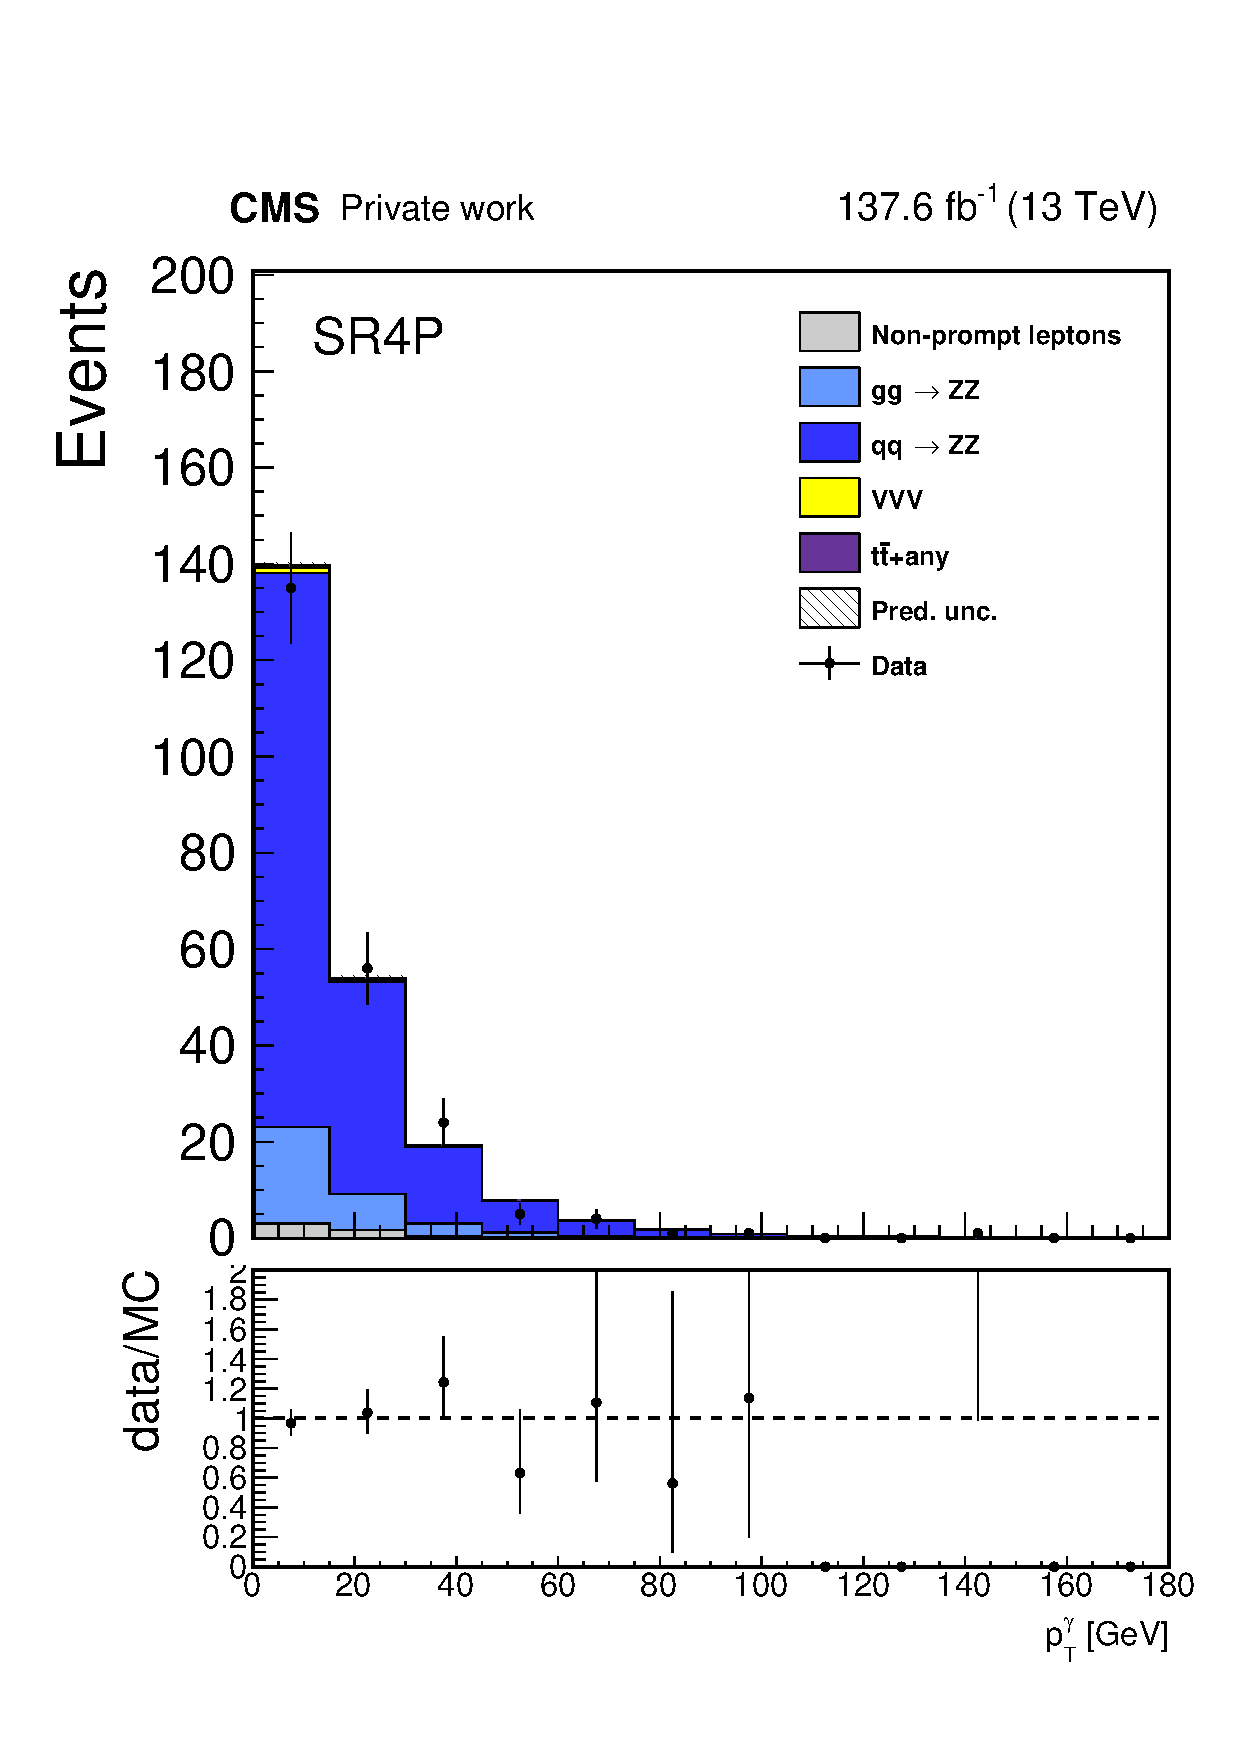
\includegraphics[width=.4\textwidth]{Figures/dataMC/Run2/lepCR/SR4P/lead_fsrPhotons_pt_pow.pdf}}
  \hfill
  \subfigure [Pseudorapidity]      {\includegraphics[width=.4\textwidth]{Figures/dataMC/Run2/lepCR/SR4P/lead_fsrPhotons_eta_pow.pdf}}
  \hfill\mbox{}
  \caption{Transverse momentum and pseudorapidity distributions of FSR photons associated to a lepton in the inclusive region with four charged leptons for \RunII.}
  \label{fig:distributions_fsrPhotons}
\end{figure}

%% \begin{figure}
%% \begin{center}
%%         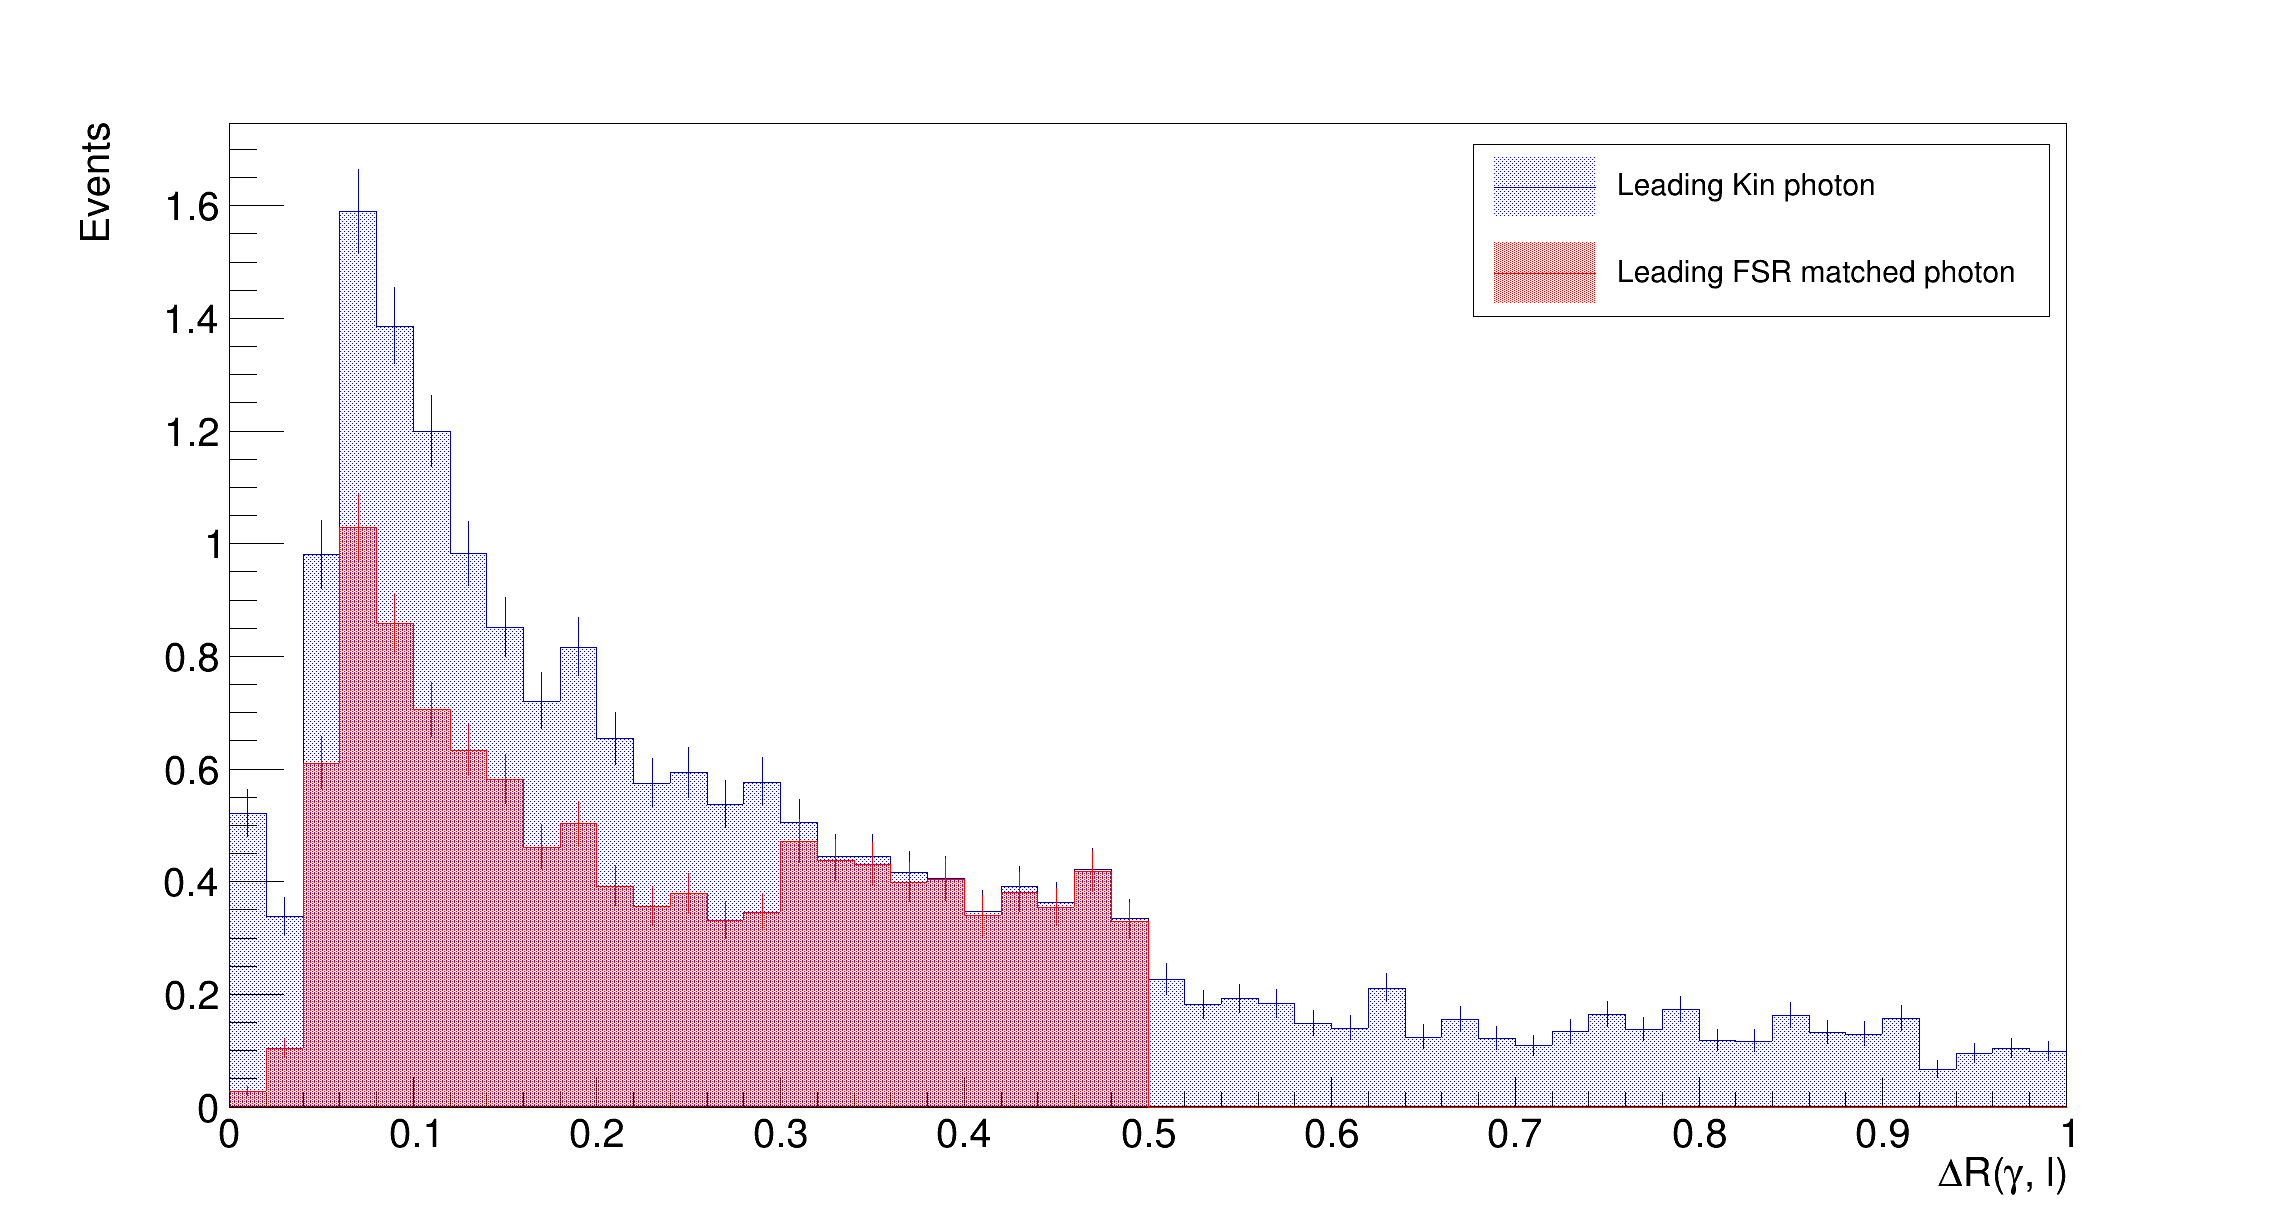
\includegraphics[width=0.8\textwidth]{Figures/lead_dRl_kin_vs_fsrMatched_rebinned.png}
%% \end{center}
%% \caption{$\Delta R(\ell, \gamma)$ for all the photons passing at least the `kinematic' selection with the $\Delta R$ cut relaxed, and for those selected as FSR in the ZZ$\gamma$ sample 2018.}
%% \label{fig:dRl_fsr_photons}
%% \end{figure}

% and the effect of not excluding FSR photons from the computation of the nonprompt rate


\subsection{Electrons}
\subsubsection{Isolation Optimization}
\label{sec:eleiso}
The electron isolation is archieved through the use of the Particle Flow relative isolation,
which is defined as:
\begin{equation}
\text{RelPFiso} = (\sum_{\text{charged}} \ET + \sum^{\text{corr}}_{\text{neutral}} \ET)/\ET^{\,\Pe}
\label{eqn:elepfrelisoeqn}
\end{equation}
To mitigate the contribution from \pileup, only charged hadrons from the primary vertex are included,
while the corrected neutral component of isolation is then computed using the formula:
\begin{equation}
\label{eqn:neutralea}
  \sum^{\text{corr}}_{\text{neutral}} \ET = \text{max} \left(0,\, \sum^{\text{uncorr}}_{\text{neutral}} \ET + \sum_{\text{photons}} \ET - \ET^\text{PU} \right)
\end{equation}
The contribution from neutral \pileup{} is estimated using:
\begin{equation}
  \ET^{PU} =  \rho \times A_\text{eff}
\label{eqn:purho}
\end{equation}
where $\rho$ is the mean energy density, estimated as the median of the distribution of the transverse energy density per unit area of \pileup{} jets in the event, $\pt^\text{jet}/A_\text{jet}$,
while the effective area $A_{\text{eff}}$ is the geometric area of the isolation cone,
corrected by an $\eta$-dependent factor to account for the dependence of the \pileup{} energy density~\cite{CMS-EGM-13-001}.

%% was optimized in Ref.~\cite{AN-15-277} and the electron isolation working was
The threshold for the electron isolation,
calculated within a cone of radius $\DR = 0.3$
is chosen to be $\text{RelPFiso} < 0.35$. 

\subsubsection{Impact Parameter Selection}
\label{sec:eleSIP}
In order to ensure that the electron trajectories are consistent with a common primary vertex
they are required to have an associated track with a small impact parameter with respect to the event primary vertex.
The significance of the impact parameter (SIP) is used:
\begin{equation}
\label{eq:SIP3D}
\SIPthreeD \mathdefined \frac{|\rm IP_{3D}|}{\sigma_{\rm IP}} \ ,
\end{equation}
where ${\rm IP_{3D}}$ is the lepton impact parameter in three dimensions,
that is the distance with respect to the primary interaction vertex the point of closest approach,
and $\sigma_{\rm IP}$ the associated uncertainty.
Electrons for the analysis must satisfy $\SIPthreeD < 4$.

\subsubsection{Electron MVA}
\label{sec:eleMVA}
Reconstructed electrons are identified and isolated by means of a Gradient Boosted Decision Tree (GBDT) multivariate classifier algorithm,
which exploits observables from the electromagnetic cluster, the matching between the cluster and the electron track, observables based exclusively on tracking measurements as well as particle flow isolation sums.
It was developed for the $\PH \to \PZ \PZ^{*} \to 4 \Pl$ analysis~\cite{CMS-HIG-19-001}
and trained separately for each data taking year on a Drell-Yan plus jets MC sample.
The classifier is trained with the e\textbf{X}treme \textbf{G}radient \textbf{Boost}ing (XGBoost) optimized distributed gradient boosting library~\cite{Chen_2016}
designed to be highly efficient, flexible and portable.

% The MVA values are userFloat("ElectronMVAEstimatorRun2Summer16ULIdIsoValues"), and the cut is done in ZZAnalysis/AnalysisStep/plugins/EleFiller.cc
The full list of observables used can be found in the Table~\ref{tab:ele_ID_input_variables}.

\begin{table}[ht]
  \caption{Overview of input variables to the multivariate classifier used to identity electrons.}
  \label{tab:ele_ID_input_variables}
  \small
  \centering
  \resizebox{\textwidth}{!}{
  \begin{tabular}{c l}
    \toprule
    Observable type & Observable name \\
    \midrule
    \multirow{6}{*}{Cluster shape}
      & RMS of the energy-crystal number spectrum: $\sigma_{i\eta i\eta}$, $\sigma_{i\varphi i\varphi}$ \\
      & Super cluster width along $\eta$ and $\phi$ \\
      & Ratio of the hadronic energy behind the SC to the SC energy, $H/E$ \\
      & Circularity $(E_{5\times5} - E_{5\times1})/E_{5\times5}$ \\
      & Sum of the seed and adjacent crystal over the SC energy $R_{9}$ \\
      & For endcap training bins: energy fraction in pre-shower $E_\text{PS}/E_\text{raw}$ \\
    \hline
    \multirow{2}{*}{Track-cluster match}
      & Energy-momentum agreement $E_{tot}/p_{in}$, $E_{ele}/p_{out}$, $1/E_{tot} - 1/p_{in}$ \\
      & Position matching $\Delta\eta_{in}$, $\Delta\varphi_{in}$, $\Delta\eta_{seed}$ \\
    \hline
    \multirow{2}{*}{Tracking}
      & Fractional momentum loss $f_{brem} = 1 - p_{out}/p_{in}$ \\
      & Reduced $\chi^2$ of the KF and GSF track $\chi^{2}_{KF}$, $\chi^{2}_{\textrm{GSF}}$ \\
    \bottomrule
  \end{tabular}
  }
\end{table}


The model is trained on 2016, 2017, and 2018 Drell-Yan with jets MC sample for both signal and background. The separate training for three periods guarantees
optimal performance during the entire \RunII{} data taking period.


Tables~\ref{tab:ele_ID_WPA}, \ref{tab:ele_ID_WPB} and~\ref{tab:ele_ID_WPC} list the cuts values applied to the MVA output for 2016, 2017, 2018 training, respectively.
For 2018, the corresponding signal and background efficiencies are given as examples.
They are very similar for 2016 and 2017.

For the analysis, loose electrons have to pass this MVA identification and isolation working point.

\begin{table}
  \caption{Minimum BDT score required for passing the electron identification, for 2016 samples.}
  \label{tab:ele_ID_WPA}
  \centering
  \begin{tabular}{c c c c}
    \toprule    %----------------------------------------------------------------------------------------
    \pt range           & $|\eta| < 0.8$ & $0.8 < |\eta| < 1.479$ & $|\eta| > 1.479$ \\
    \midrule    %----------------------------------------------------------------------------------------
    $5 < \pt < 10 \GeV$ &  0.9503        &  0.9461                &  0.9387 \\
    $\pt > 10 \GeV$     &  0.3782        &  0.3587                & -0.5745 \\
    \bottomrule %----------------------------------------------------------------------------------------
  \end{tabular}
\end{table}

\begin{table}
  \caption{Minimum BDT score required for passing the electron identification, for 2017 samples.}
  \label{tab:ele_ID_WPB}
  \centering
  \begin{tabular}{c c c c}
    \toprule    %----------------------------------------------------------------------------------------
    \pt range           & $|\eta| < 0.8$ & $0.8 < |\eta| < 1.479$ & $|\eta| > 1.479$ \\
    \midrule    %----------------------------------------------------------------------------------------
    $5 < \pt < 10 \GeV$ &  0.8521        &  0.8268                &  0.8694 \\
    $\pt > 10 \GeV$     &  0.9825        &  0.9692                &  0.7935 \\
    \bottomrule %----------------------------------------------------------------------------------------
  \end{tabular}
\end{table}

\begin{table}
  \caption{Minimum BDT score required for passing the electron identification and corresponding signal and background efficiencies, for 2018 samples.}
  \label{tab:ele_ID_WPC}
  \centering
  \begin{tabular}{c c c c c}
    \toprule
    $|\eta|$ range                      & \pt range           & Cut on BDT & Signal eff. & Background eff. \\
    \midrule
    \multirow{2}{*}{$|\eta| < 0.8 $}    & $5 < \pt < 10 \GeV$ &  0.8956    &  81.0\,\%   &  4.4\,\% \\
                                        & $\pt > 10 \GeV$     &  0.0424    &  97.1\,\%   &  2.9\,\% \\
    \hline
    \multirow{2}{*}{$0.8<|\eta|<1.479$} & $5 < \pt < 10 \GeV$ &  0.9111    &  79.3\,\%   &  4.6\,\% \\
                                        & $\pt > 10 \GeV$     &  0.0047    &  96.3\,\%   &  3.6\,\% \\
    \hline
    \multirow{2}{*}{$|\eta| > 1.479$}   & $5 < \pt < 10 \GeV$ &  0.9401    & 73.0\,\%    &  3.6\,\% \\
                                        & $\pt > 10 \GeV$     & -0.6042    & 95.7\,\%    &  6.7\,\% \\
    \bottomrule
  \end{tabular}
\end{table}

\subsubsection{Analysis selection for electrons}%% {Electron Selection}
\label{sec:ele_selection}
Electron candidates are preselected using loose cuts on track-cluster matching observables, so as to preserve the highest possible efficiency while rejecting part of the QCD background. To be considered for the analysis, electrons are required to have a
transverse momentum $p^e_T >$ 7 GeV, a reconstructed $|\eta^e| <$ 2.5, and to satisfy a loose primary vertex
constraint defined as $d_{xy} < 0.5$ cm and $d_z < 1$ cm.
Such electrons are called {\bf loose electrons}.

The data-MC discrepancy is corrected using scale factors as is done for the electron selection with data efficiencies measured using the same tag-and-probe technique outlined later (see Section~\ref{sec:eleEffMeas}).
These studies for reconstructions are carried out by the EGM POG and the results are only summarised here.

The electron reconstruction scale factors
% are shown Fig.~\ref{fig:ele_rec_scale_factors} and
are applied as a function of the super cluster $\eta$ and electron $\pt$.


\subsection{Muons}
\subsubsection{Muon Isolation}
\label{sec:muoniso}
A Particle Flow based isolation is used to suppress the contamination from muon from hadronic decays inside jets.
The so-called $\Delta\beta$ correction is applied in order to subtract the \pileup{} contribution for the muons, 
whereby $\Delta\beta = \frac{1}{2} \sum^\text{charged had.}_\text{PU} \pt$
gives an estimate of the energy deposit of neutral particles (hadrons and photons) from \pileup{} vertices.

The relative isolation for muons is then defined as:
\begin{equation}
\text{RelPFIso} = \frac{1}{\pt^\text{muon}} \left( \sum_\text{charged had.} \pt + \max(0, \sum_\text{neutral had.} \ET + \sum_\text{photon} \ET - \Delta \beta) \right)
\label{eqn:mupfiso}
\end{equation}

where the sums run over the photons, charged and neutral hadrons in a cone with $\DR = 0.3$ around the muon.
Only charged hadrons originating from the primary vertex are included to minimise the \pileup{} contribution.

The isolation cone for muons was optimised and the working point was chosen to be $\text{RelPFiso}(\Delta R = 0.3) < 0.35$. 

Similarly to electrons, a condition on the significance of the 3D impact parameter (\SIPthreeD, see Equation \ref{eq:SIP3D}) is applied,
in order to ensure that muons are consistent with the primary vertex.
Muons are required to satisfy $\SIPthreeD < 4$.

\subsubsection{Muon Identification}
%More details on muon reconstruction can be found in Ref.~\cite{AN-15-277}.
The analysis definition of {\bf loose muons} requires
$p_T > 5$, $|\eta| < 2.4$, $dxy< 0.5$ cm, $dz < 1$ cm, where $dxy$ and $dz$ are 
defined w.r.t. the PV and using the 'muonBestTrack'. Muons have to be 
reconstructed by either the Global Muon or Tracker Muon algorithm. Standalone 
Muon tracks that are only reconstructed in the muon system are rejected.
Muons with \verb|muonBestTrackType==2| (standalone) are discarded even if they 
are marked as global or tracker muons. 

Loose muons with $\pt$ below 200\GeV that also pass
%Muon BDT (see below).
the PF loose muon ID are considered {\bf tight muons} for this analysis.
Note that the naming convention used for these IDs differs from the muon POG
naming scheme, in which the ``tight ID'' used here is called the ``loose ID''.

Those with $\pt$ above 200\GeV are considered tight if they pass
either the PF ID or the Tracker
High-$\pt$ ID, the definition of which is shown in Table~\ref{tab:highPtID}.
This relaxed definition is used to increase signal efficiency in the high
centre of mass energy regime.
% This relaxed definition is used to increase signal efficiency for the high-mass
% search. When a very heavy resonance decays to two $\cPZ$ bosons, both bosons
% will be very boosted.
In the lab frame, the leptons coming from the decay of
a highly boosted $\cPZ$ will be nearly collinear, and the PF ID loses 
efficiency for muons separated by approximately $\Delta R < 0.4$, which roughly 
corresponds to muons originating from $\cPZ$ bosons with $\pt > 500\GeV$.

\begin{table}[ht]
    \begin{small}
    \begin{center}
    \caption{
      The requirements for a muon to pass the Tracker High-$\pt$ ID. Note that
      these are equivalent to the Muon POG High-$\pt$ ID with the global track 
      requirements removed.
      }
    \begin{tabular}{|l|l|}
      \hline
      Plain-text description         & Technical description                 \\
      \hline
      Muon station matching          & Muon is matched to segments           \\
                                     & in at least two muon stations         \\
                                     & \textbf{NB: this implies the muon is} \\
                                     & \textbf{an arbitrated tracker muon.}  \\
      \hline                                                          
      Good $\pt$ measurement         & $\frac{\pt}{\sigma_{\pt}} < 0.3$      \\
      \hline
      Vertex compatibility ($x-y$)   & $d_{xy} < 2$~mm                       \\
      \hline
      Vertex compatibility ($z$)     & $d_{z} < 5$~mm                        \\
      \hline
      Pixel hits                     & At least one pixel hit                \\
      \hline
      Tracker hits                   & Hits in at least six tracker layers   \\
      \hline
    \end{tabular}
    \label{tab:highPtID}
    \end{center}
    \end{small}
\end{table}

An additional ``ghost-cleaning'' step is performed to deal with situations when a single muon
can be incorrectly reconstructed as two or more muons:

\begin{itemize}

\item Tracker Muons that are not Global Muons are required to be arbitrated.
\item If two muons are sharing 50\% or more of their segments then the muon with lower quality is removed.

\end{itemize}


Loose muons that pass also the identification, isolation and \SIPthreeD requirements are defined \textbf{tight muons}.

\subsection{Photon Identification}
\label{sec:photonID}
Photon candidates are required to have $E_{T} > 20 \GeV$ and be in the fiducial Barrel region or Endcap regions,
defined by $|\eta|<1.4442$ and $1.566<|\eta|<2.5$, respectively.
The photon candidates are also required to be separated from the closest lepton (electron or muon) by at least $\DR(\PGg, \Pl) > 0.5$,
which highly suppresses the contribution from FSR,
and is orthogonal to the selection used for lepton FSR recovery (see Section \ref{sec:FSRphotons}).

Different strategies are used to identify prompt (produced at the primary vertex) and isolated
electrons and photons, and separate them from background sources.
The most important background to prompt photons arises from jets fragmenting mainly into light neutral mesons
such as \Pgpz or \PGh, which promptly decay to two photons.
For the energy range of interest, the meson is significantly boosted, such that the two photons from the decay are nearly collinear
and are difficult to distinguish from a single-photon incident on the calorimeter.
%% Different working points are defined to identify either electrons or photons,
%% corresponding to identification efficiencies of approximately 70, 80, and 90 \%, respectively.
%% In all cases data and simulation efficiencies are compatible within 1-5 \% over the full $\eta$ and \ET ranges for electrons and photons.

Both a cut-based and a MVA-based ID are employed and compared in the analysis.
Each has its own advantages and disadvantages.
Due to its nature, the cut-based ID can be easily inverted by reversing only one or a few of its cuts.
On the other hand, MVA-based ID is more effective at discriminating between signal and background, providing a higher signal-to-noise ratio.

\paragraph{Identification variables\\}
One of the most efficient ways to reject photon backgrounds is the use of isolation energy sums,
a generic class of discriminating variables that are constructed from the sum of the reconstructed energy in a cone around photons in different subdetectors.
%% For this purpose, it is convenient to define cones in terms of an $\eta-\phi$ metric;
%% the distance with respect to the reconstructed photon direction is defined by \DR.
A veto region inside the cone is defined, to ensure that the energy from the photon itself is not included in this sum.

Photon isolation exploits the information provided by the PF event reconstruction (Section \ref{sec:ParticleFlow}).
The isolation variables are obtained by summing the transverse momenta of charged hadrons ($I_{ch}$), photons ($I_\PGg$), and neutral hadrons ($I_n$),
inside an isolation cone of $\DR = 0.3$ with respect to the electron or photon direction.
The larger the energy of the incoming electrons or photons, the larger the amount of energy spread around its direction in the various subdetectors.
For this reason, the thresholds applied on the isolation quantities are frequently parameterised as a function of the particle \ET.

The isolation variables are corrected to mitigate the contribution from pileup.
This contribution in the isolation region is estimated as $\rho A_{eff}$,
where $\rho$ is the median of the transverse energy density per unit area in the event
and $A_{eff}$ is the area of the isolation region weighted by a factor that accounts for the dependence of the pileup transverse energy density on the object $\eta$ \cite{CMS:electron-performance-2015}.
The quantity $\rho A_{eff}$ is subtracted from the isolation quantities.

The distributions of $I_\PGg$ before % after?
the $\rho$ corrections are shown in Figure~\ref{fig:Iph_CR2P2F} for photons in the EB and EE.

\begin{figure}
\subfigure [Barrel] {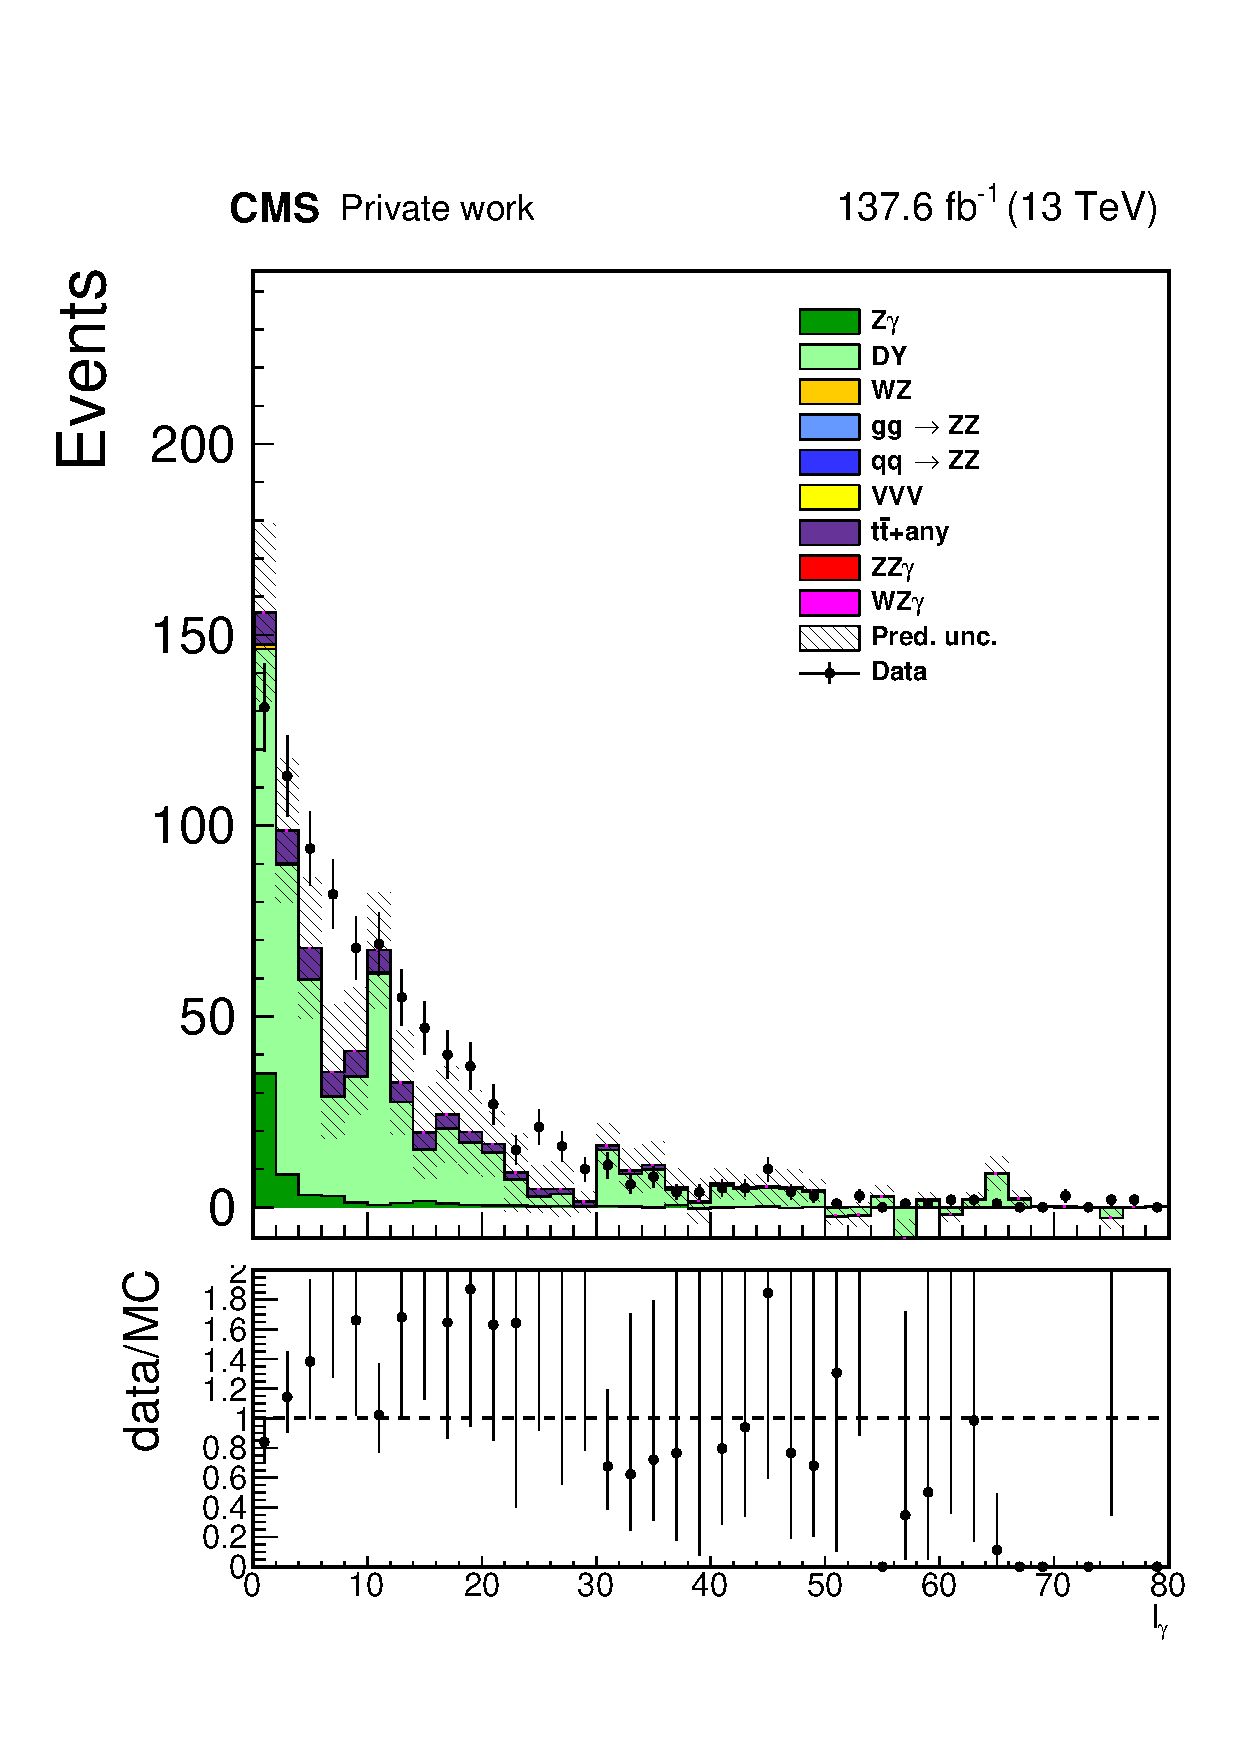
\includegraphics[width=.5\textwidth]{Figures/VVGammaAnalyzer_noLFR/Run2/fullMC/CR2P2F/kinPh_phIso_EB_pow.pdf}}%
\subfigure [Endcap] {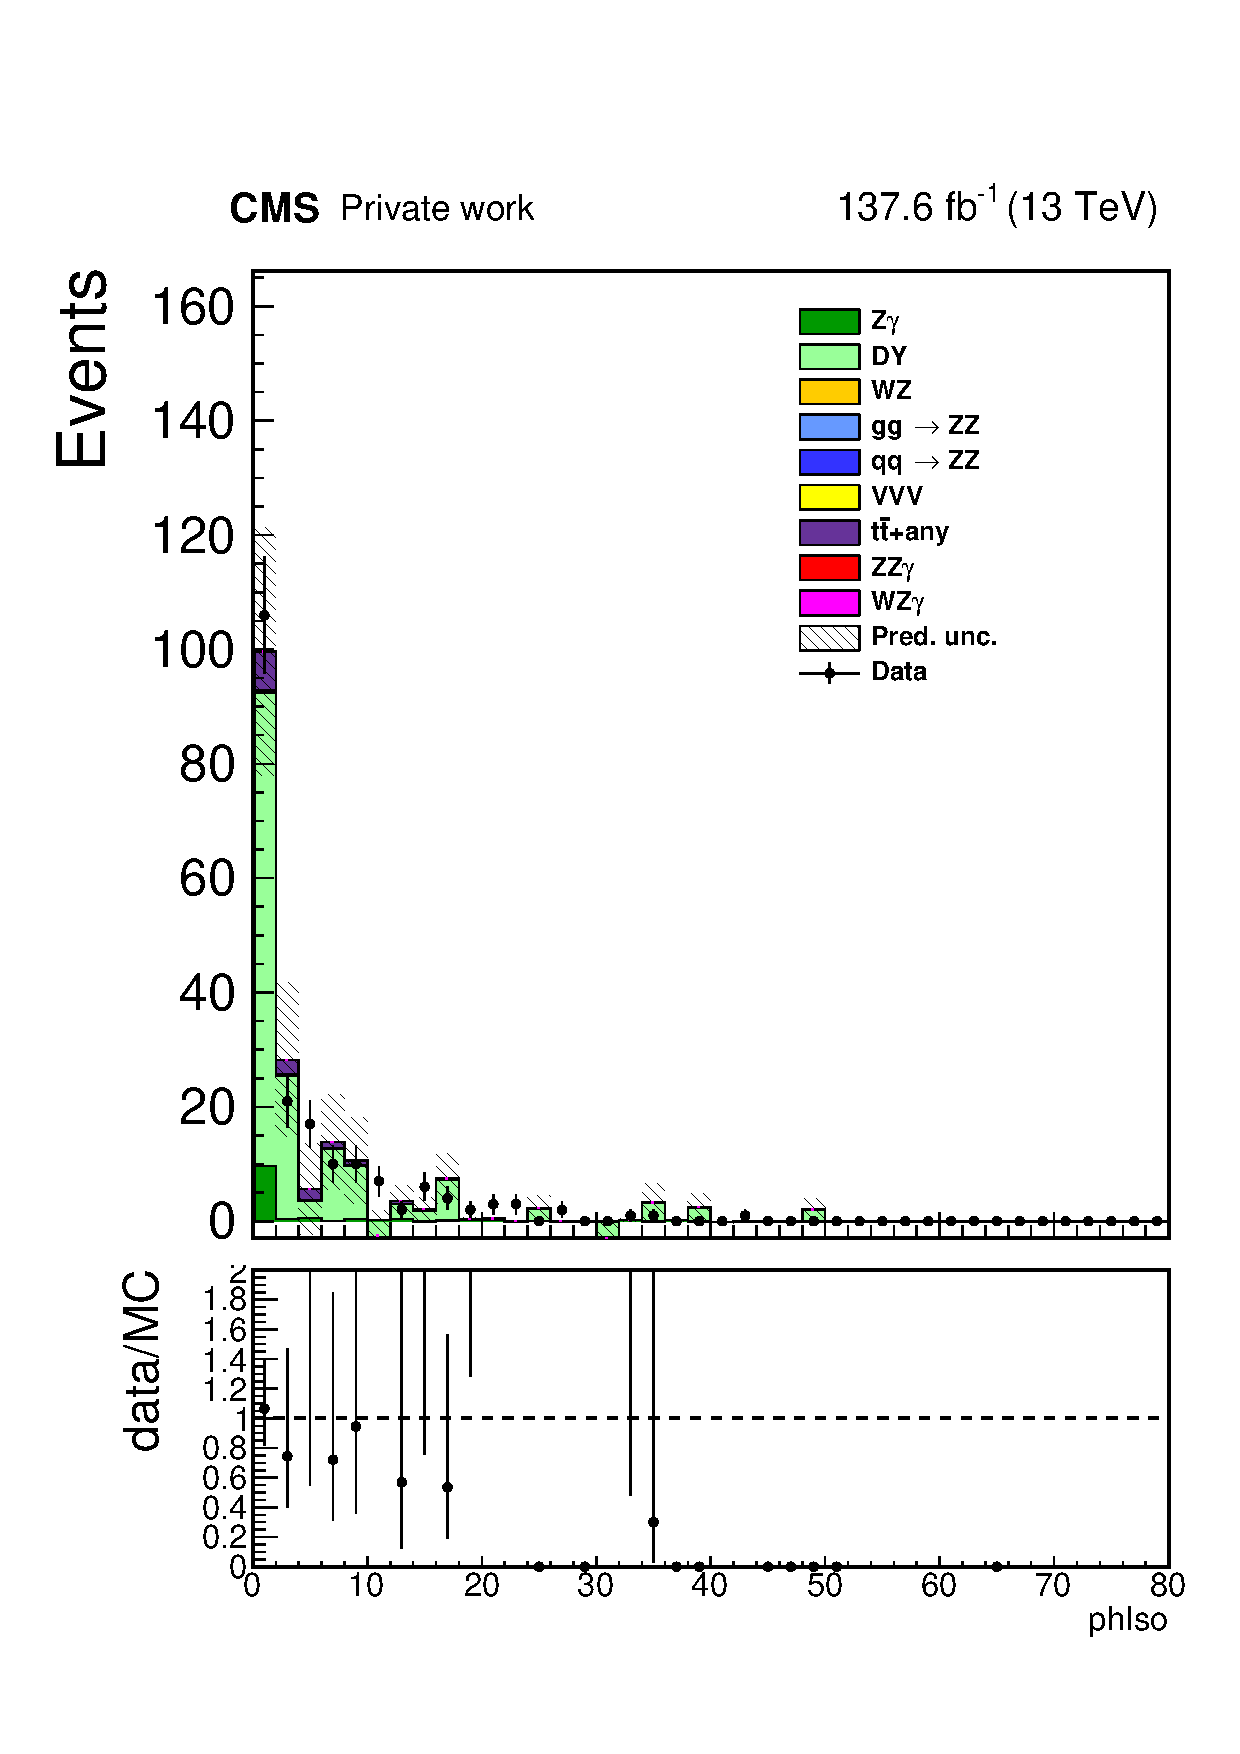
\includegraphics[width=.5\textwidth]{Figures/VVGammaAnalyzer_noLFR/Run2/fullMC/CR2P2F/kinPh_phIso_EE_pow.pdf}}
\caption{The PF photon isolation ($I_\PGg$), before the $\rho$ correction, in a cone defined by $\DR = 0.3$ for photons in the EB (left) and in the EE (right).
The events belong to the leptonic control region CR2P2F (see Section \ref{sec:fake_leptons}).
The lower panels display the ratio of the data to the simulation.}
\label{fig:Iph_CR2P2F}
\end{figure}

Another method to reject jets with high electromagnetic content exploits the shape of the electromagnetic shower in the ECAL.
Even if the two photons from neutral hadron decays inside a jet cannot be fully resolved, a wider shower profile is expected, on average,
compared with a single incident electron or photon.
This is particularly true along the $\eta$ axis of the cluster, since the presence of the material combined with the effect of the magnetic field
reduce the discriminating power resulting from the $\phi$ profile of the shower. 
In particular, the following two variables have high discriminating power.

The hadronic over electromagnetic energy ratio ($H/E$) is defined as the ratio between the energy deposited in the HCAL in a cone of radius $\DR = 0.15$
around the supercluster direction and the energy of the photon candidate.
\sieie, the second moment of the log-weighted distribution of crystal energies in $\eta$,
calculated in the $5 \times 5$ matrix around the most energetic crystal in the SC and rescaled to units of crystal size.
The mathematical expression is given below:
\begin{equation}
\label{eq:sieie}
\sieie \mathdefined \sqrt{ \frac{\sum_i^{5 \times 5} w_i(\eta_i - \bar{\eta}_{5 \times 5})}{\sum_i^{5 \times 5} w_i} }
\end{equation}
where $\eta_i$ is the pseudorapidity of the i-th crystal,
$\bar{\eta}_{5 \times 5}$ is the mean pseudorapidity of the $5 \times 5$ cells
and $w_i$ is a weight defined as $w_i = \mathrm{max}(0,\, 4.7 + \mathrm{ln}(E_i/E_{5 \times 5}))$,
which is nonzero if $E_i > 0.9\, \%\; E_{5 \times 5}$.
Looking at the numerator in Equation \ref{eq:sieie}, it is clear that \sieie is proportional to the distance between adjacent crystals,
which is 0.0175 in EB and varies from 0.0175 to 0.0 in EE.
Therefore, the spread of \sieie in EE is twice the one in EB.
The \sieie distribution is expected to be narrow for isolated electrons or photons, and broad for two-photon showers from meson decays.
The distributions of \sieie are shown in Figure \ref{fig:sieie_CR2P2F} for photons in the EB and EE.

\begin{figure}
\subfigure [Barrel] {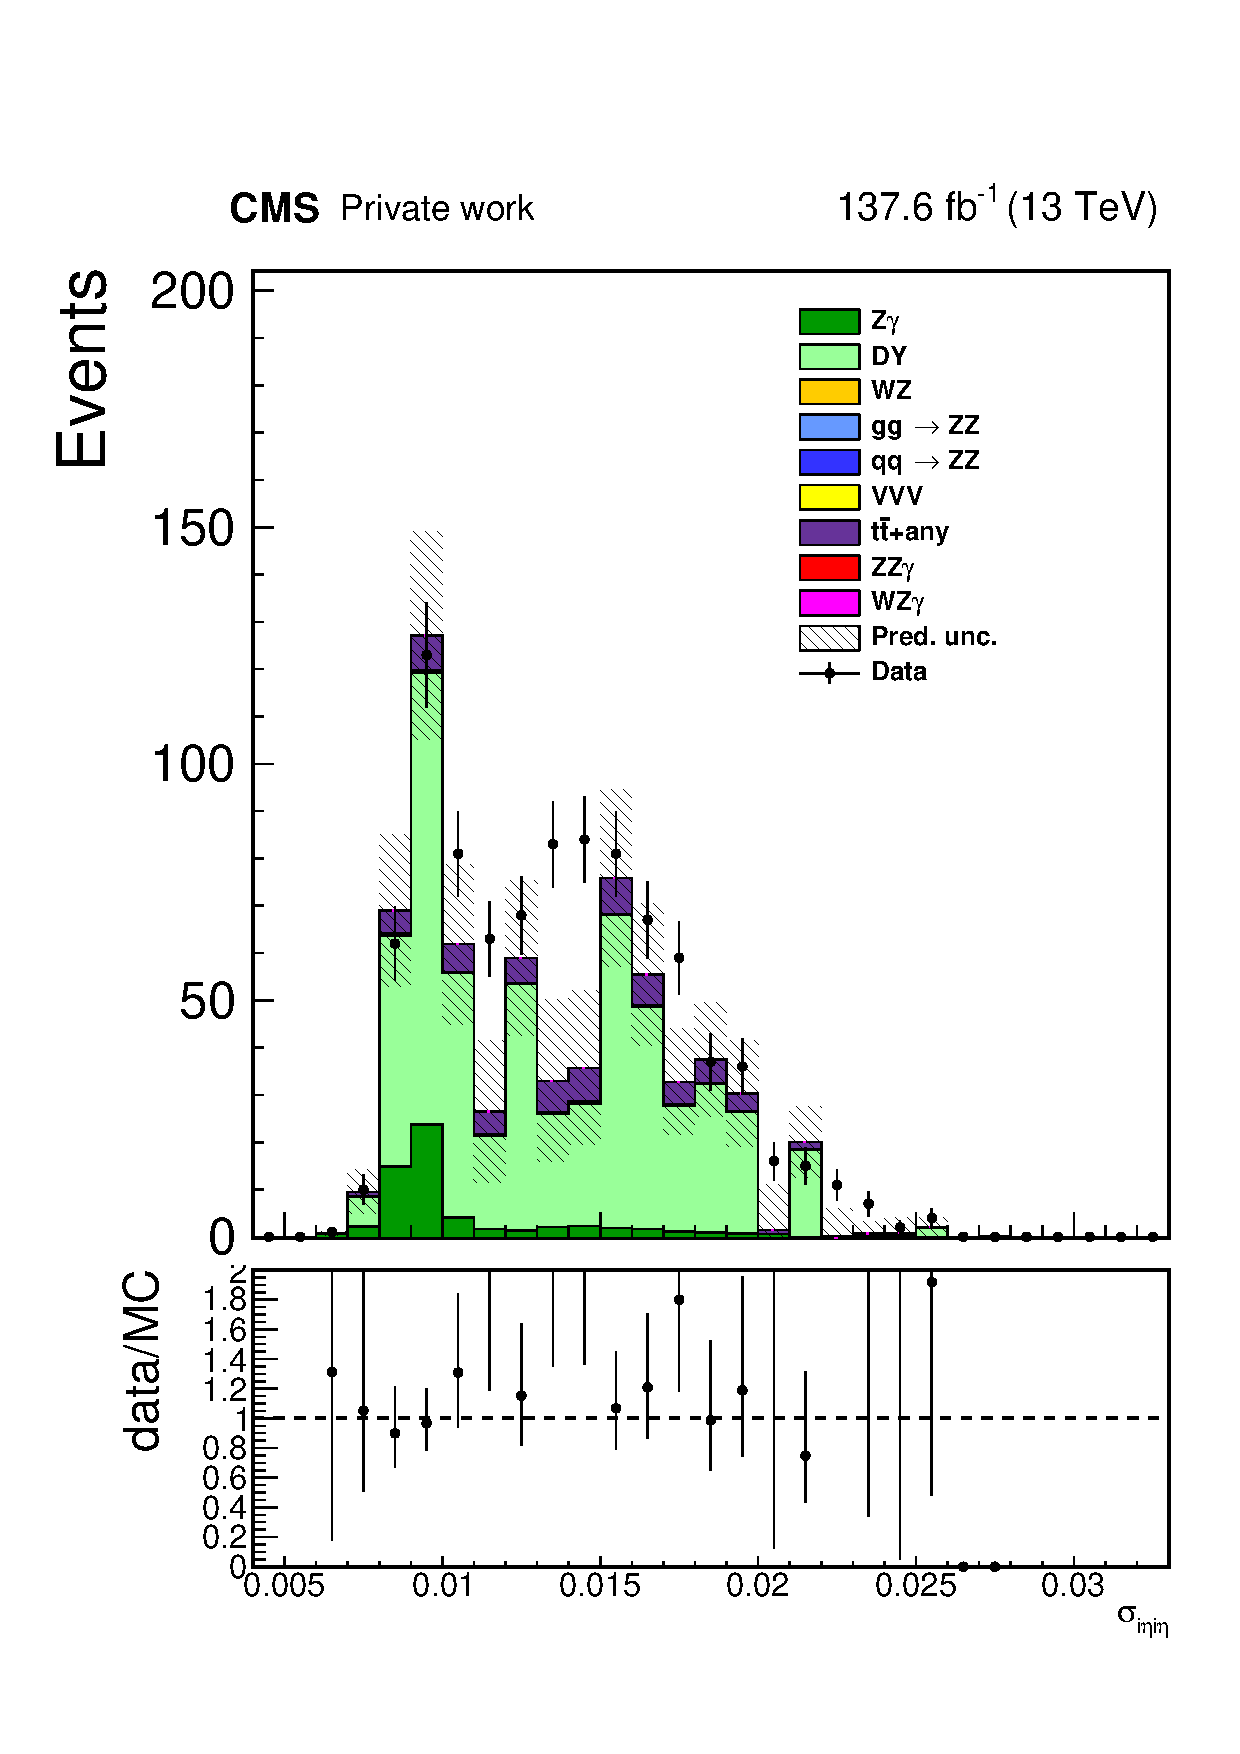
\includegraphics[width=.5\textwidth]{Figures/VVGammaAnalyzer_noLFR/Run2/fullMC/CR2P2F/kinPh_sieie_EB_pow.pdf}}%
\subfigure [Endcap] {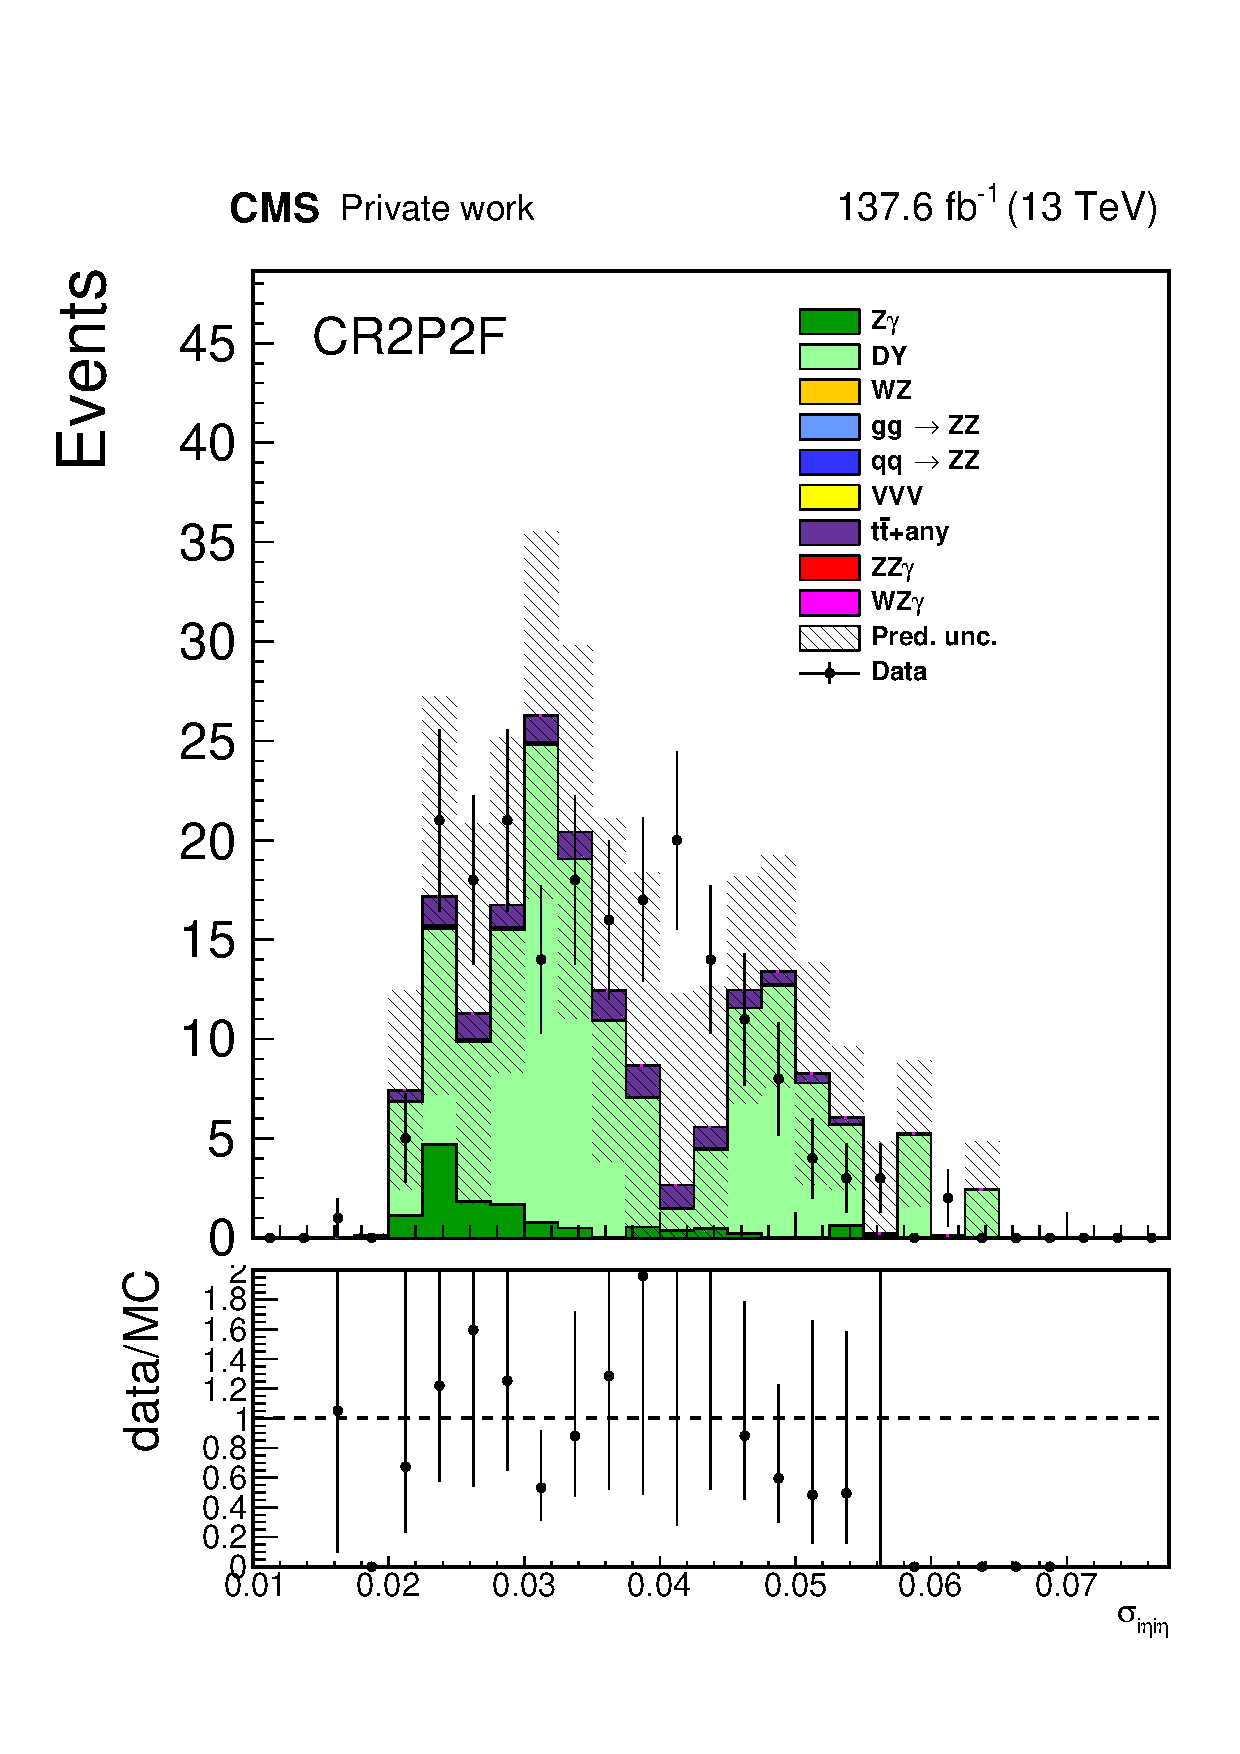
\includegraphics[width=.5\textwidth]{Figures/VVGammaAnalyzer_noLFR/Run2/fullMC/CR2P2F/kinPh_sieie_EE_pow.pdf}}
\caption{Distribution of \sieie for photons in the EB (left) and in the EE (right).
The events belong to the leptonic control region CR2P2F (see Section \ref{sec:fake_leptons}).
The lower panels display the ratio of the data to the simulation.}
\label{fig:sieie_CR2P2F}
\end{figure}

Another important variable is $R_9$, which is defined as the ratio between the energy contained in the $3 \times 3$ array of crystals,
centered around the most energetic crystal of the SC,
to the total energy of the supercluster.

\paragraph{Cut-based ID\\}
The cut-based photon ID~\cite{CMS:EGM-17-001} uses 5 variables: $H/E$, \sieie, $I_{ch}^{corr}$, $I_{n} ^{corr}$ and $I_{\PGg} ^{corr}$.
The Loose working point, shown in Table~\ref{tab:VPhotonID}, is selected for this analysis.
It provides 90\,\% efficiency on signal photons with 86\,\% (77\,\%) background rejection in the Barrel (Endcap).
The efficiency in data is well modelled in simulation, and the ratio between the two, shown in Figure \ref{fig:phEffSF}, is within 5\,\% from unity.
This ratio is referred as Scale Factor (SF), and is applied to simulation to correct for the residual mismodelling and avoid biasing the results.

\begin{table}
  \centering
  \renewcommand{\arraystretch}{1.4}
  \begin{tabular}{c c c}
    \toprule
    Variable                 &  Barrel $\quad |\eta| < 1.4442$     & Endcap $\quad 1.566 < |\eta| < 2.5$\\
    \midrule
    $H/E$                    & $0.04596$                           & $0.0590$                           \\
    $\sigma_{i\eta i\eta}$   & $0.0106$                            & $0.0272$                           \\
    $I_{ch}^{corr} [\GeV]$   & $1.694$                             & $2.089$                            \\
    $I_{n} ^{corr} [\GeV]$   & \renewcommand{\arraystretch}{1}\begin{tabular}{c} $24.032 + 0.01512\, p_{T}^{\gamma} +$\\$+ 2.259 \cdot 10^{-5}\, (p_{T}^{\gamma})^2$ \end{tabular}
                             & \renewcommand{\arraystretch}{1}\begin{tabular}{c} $19.722 + 0.0117\, p_{T}^{\gamma} +$ \\$+ 2.3 \cdot 10^{-5}\, (p_{T}^{\gamma})^2$   \end{tabular}\\
    $I_{\PGg}^{corr} [\GeV]$ & $2.876 + 0.004017\, p_{T}^{\gamma}$ & $4.162 + 0.0037\, p_{T}^{\gamma}$  \\
    \bottomrule
  \end{tabular}
  \caption[.]{Cut thresholds of the Loose working point cut-based photon ID.}
  \label{tab:VPhotonID}
\end{table}

\begin{figure}
  \subfigure [2016preVFP ] {\resizebox{.5\textwidth}{!}{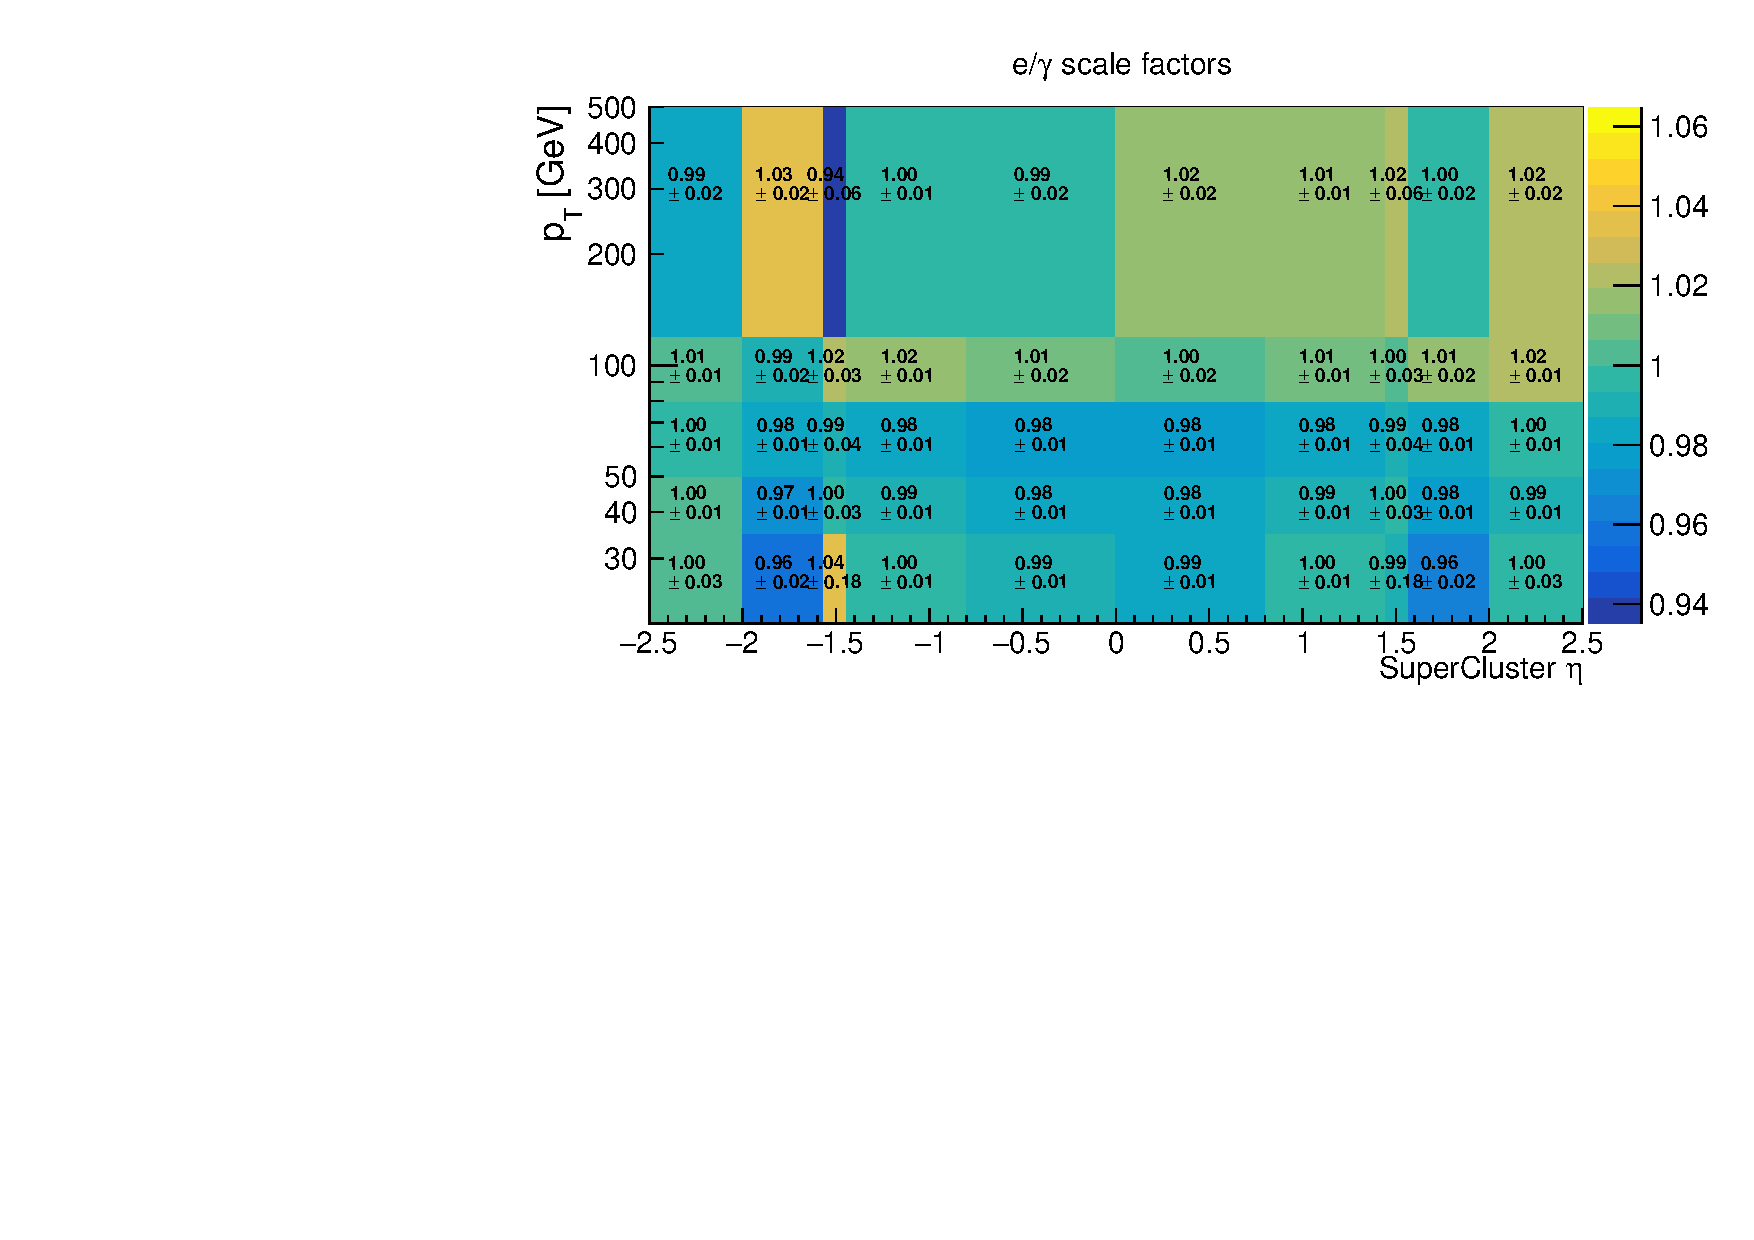
\includegraphics[width=.5\textwidth]{SF/phEffSF_2016preVFP.pdf} }}
  \subfigure [2016postVFP] {\resizebox{.5\textwidth}{!}{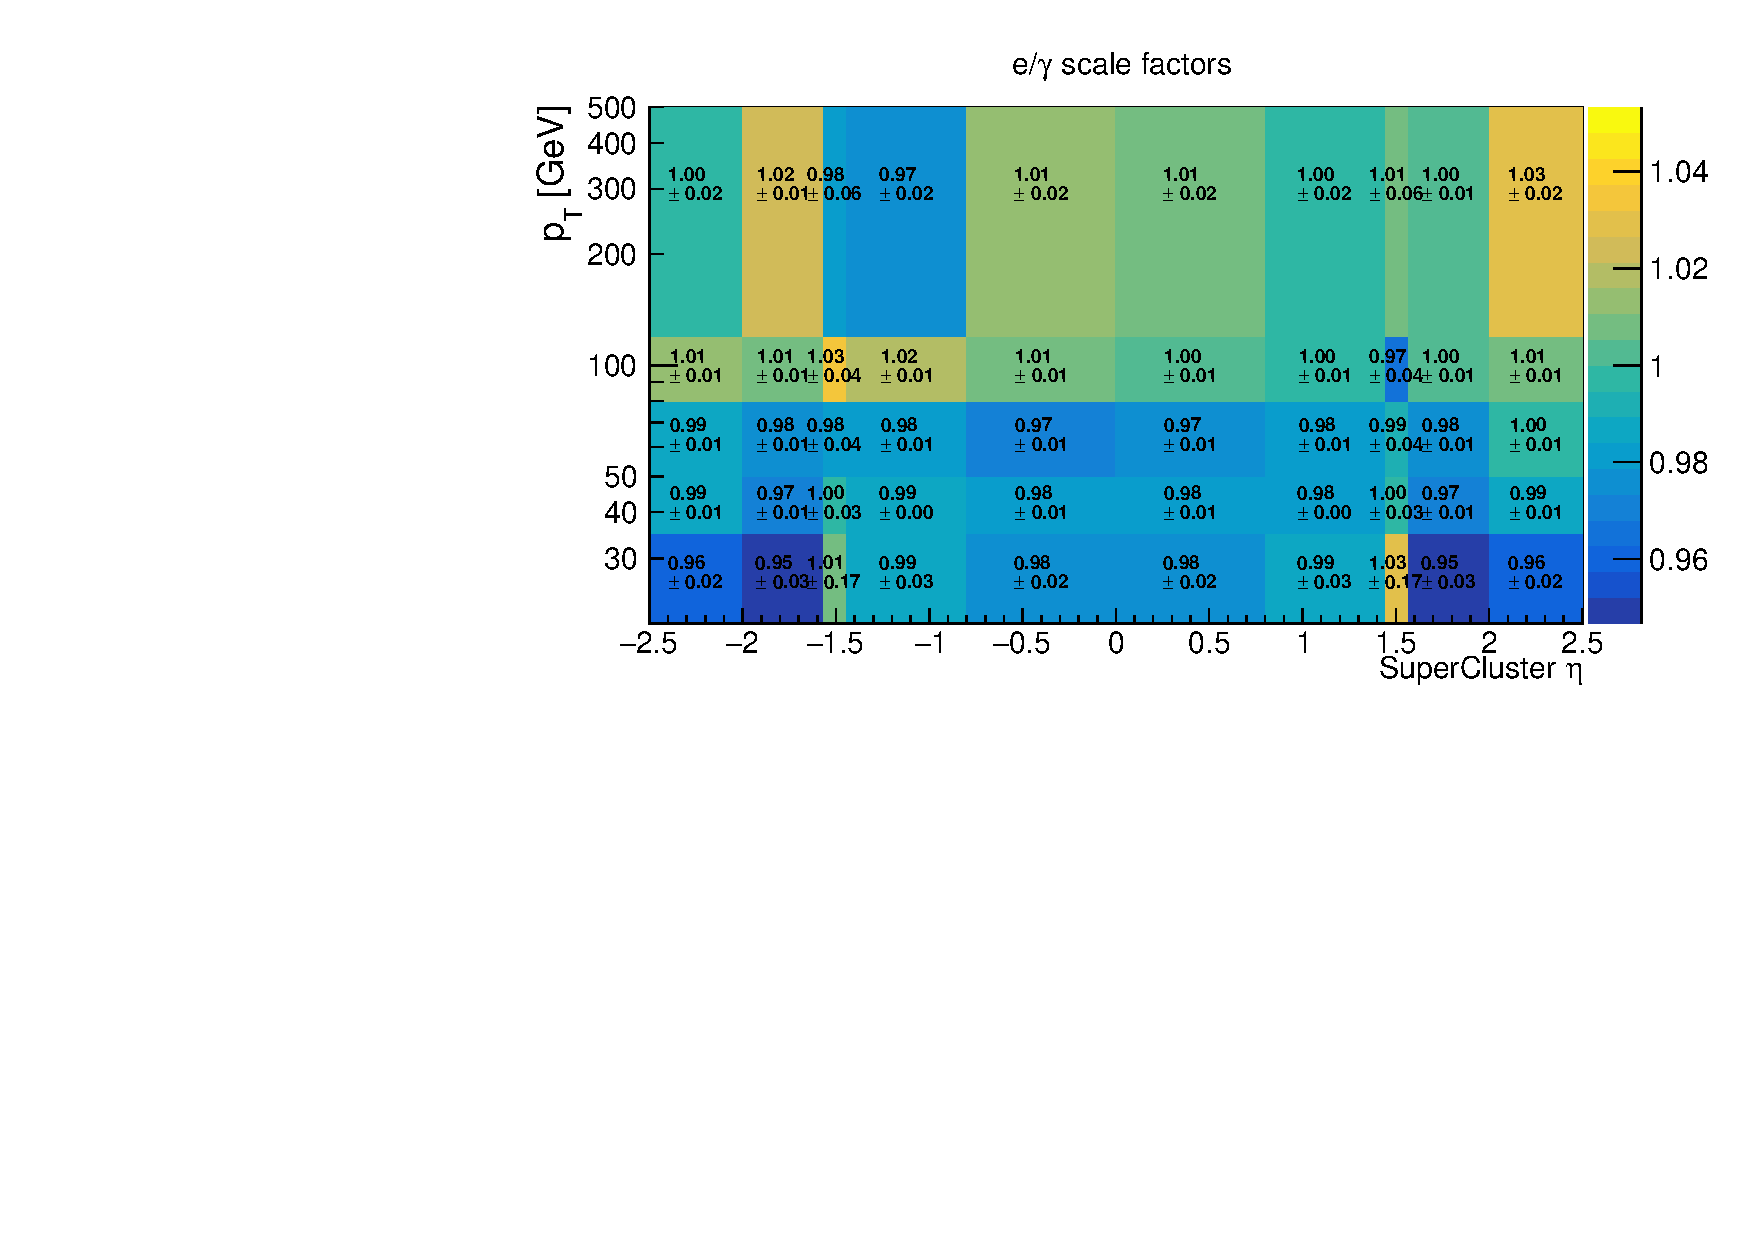
\includegraphics[width=.5\textwidth]{SF/phEffSF_2016postVFP.pdf}}}\\
  \subfigure [2017]        {\resizebox{.5\textwidth}{!}{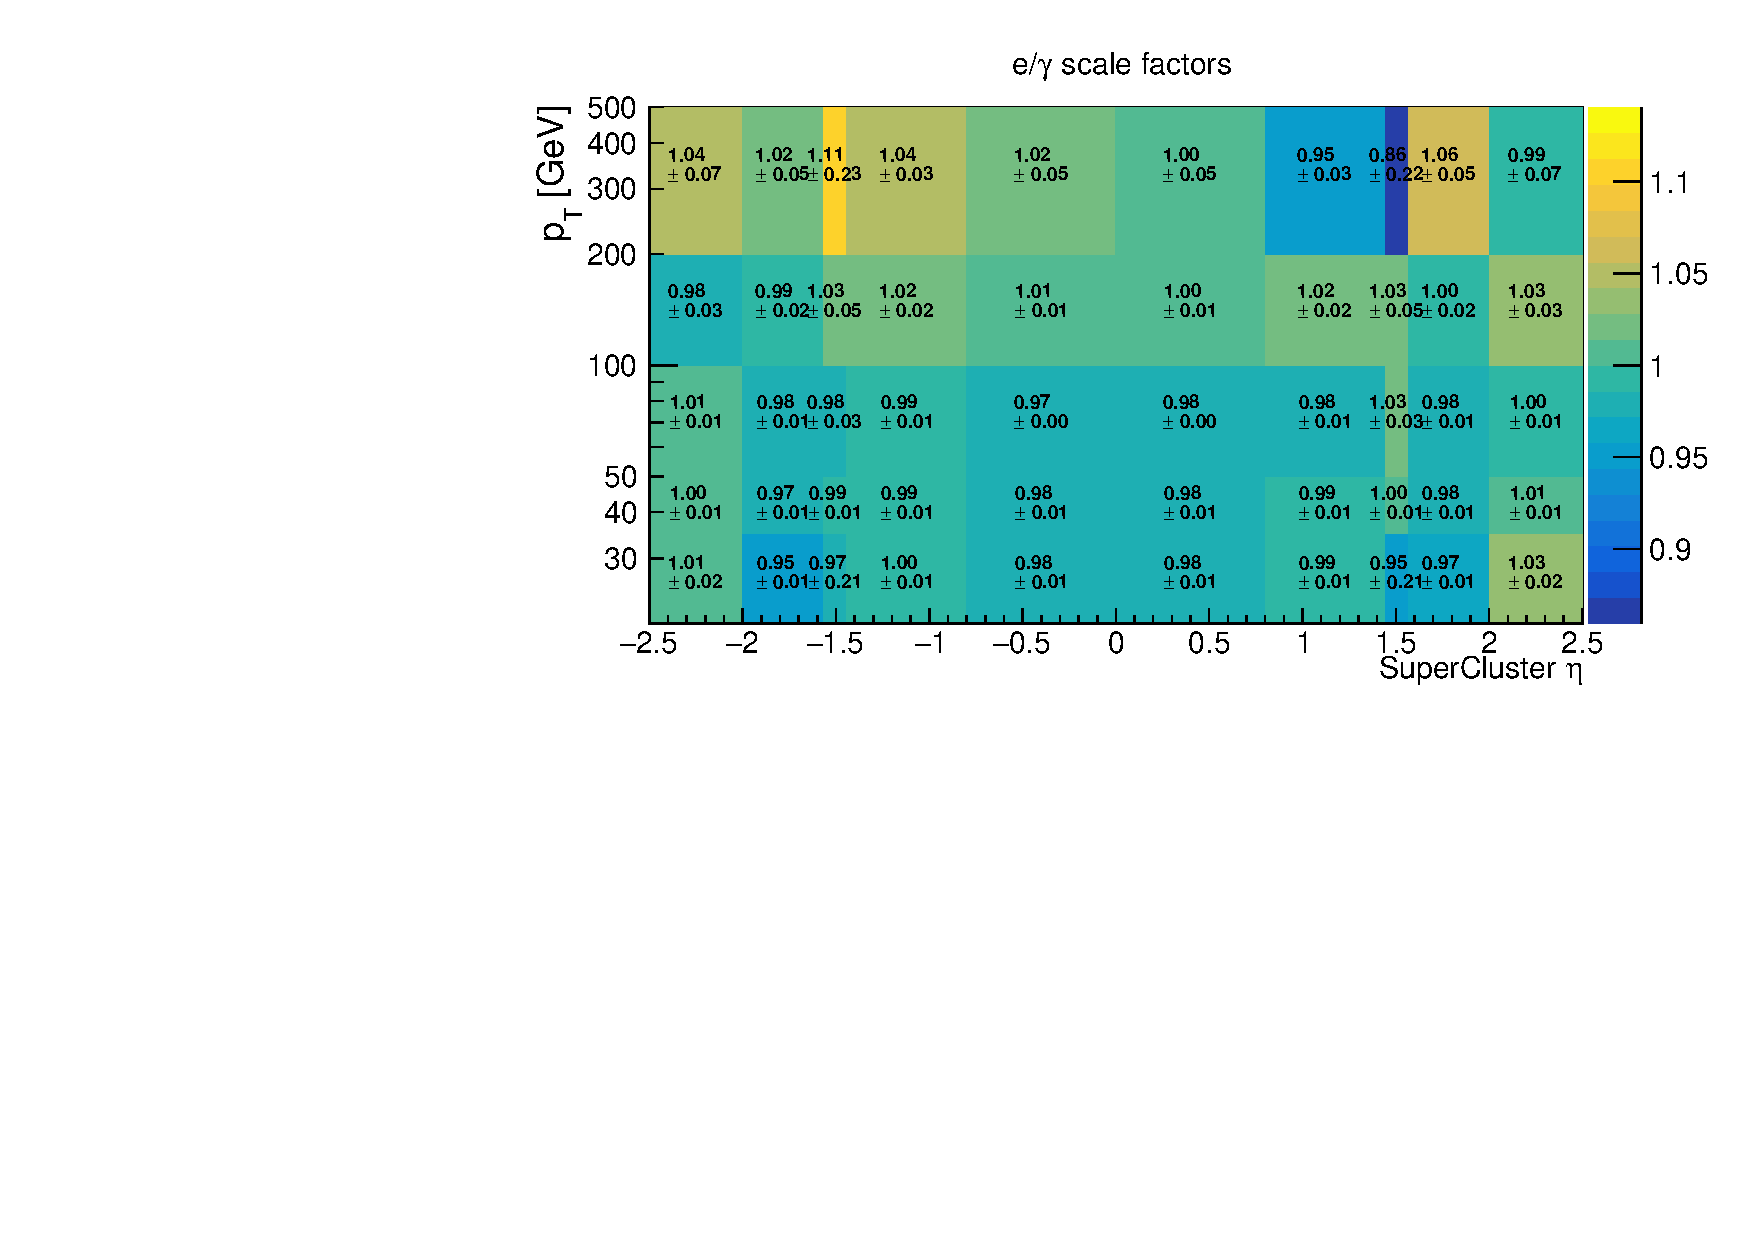
\includegraphics[width=.5\textwidth]{SF/phEffSF_2017.pdf}}}
  \subfigure [2018]        {\resizebox{.5\textwidth}{!}{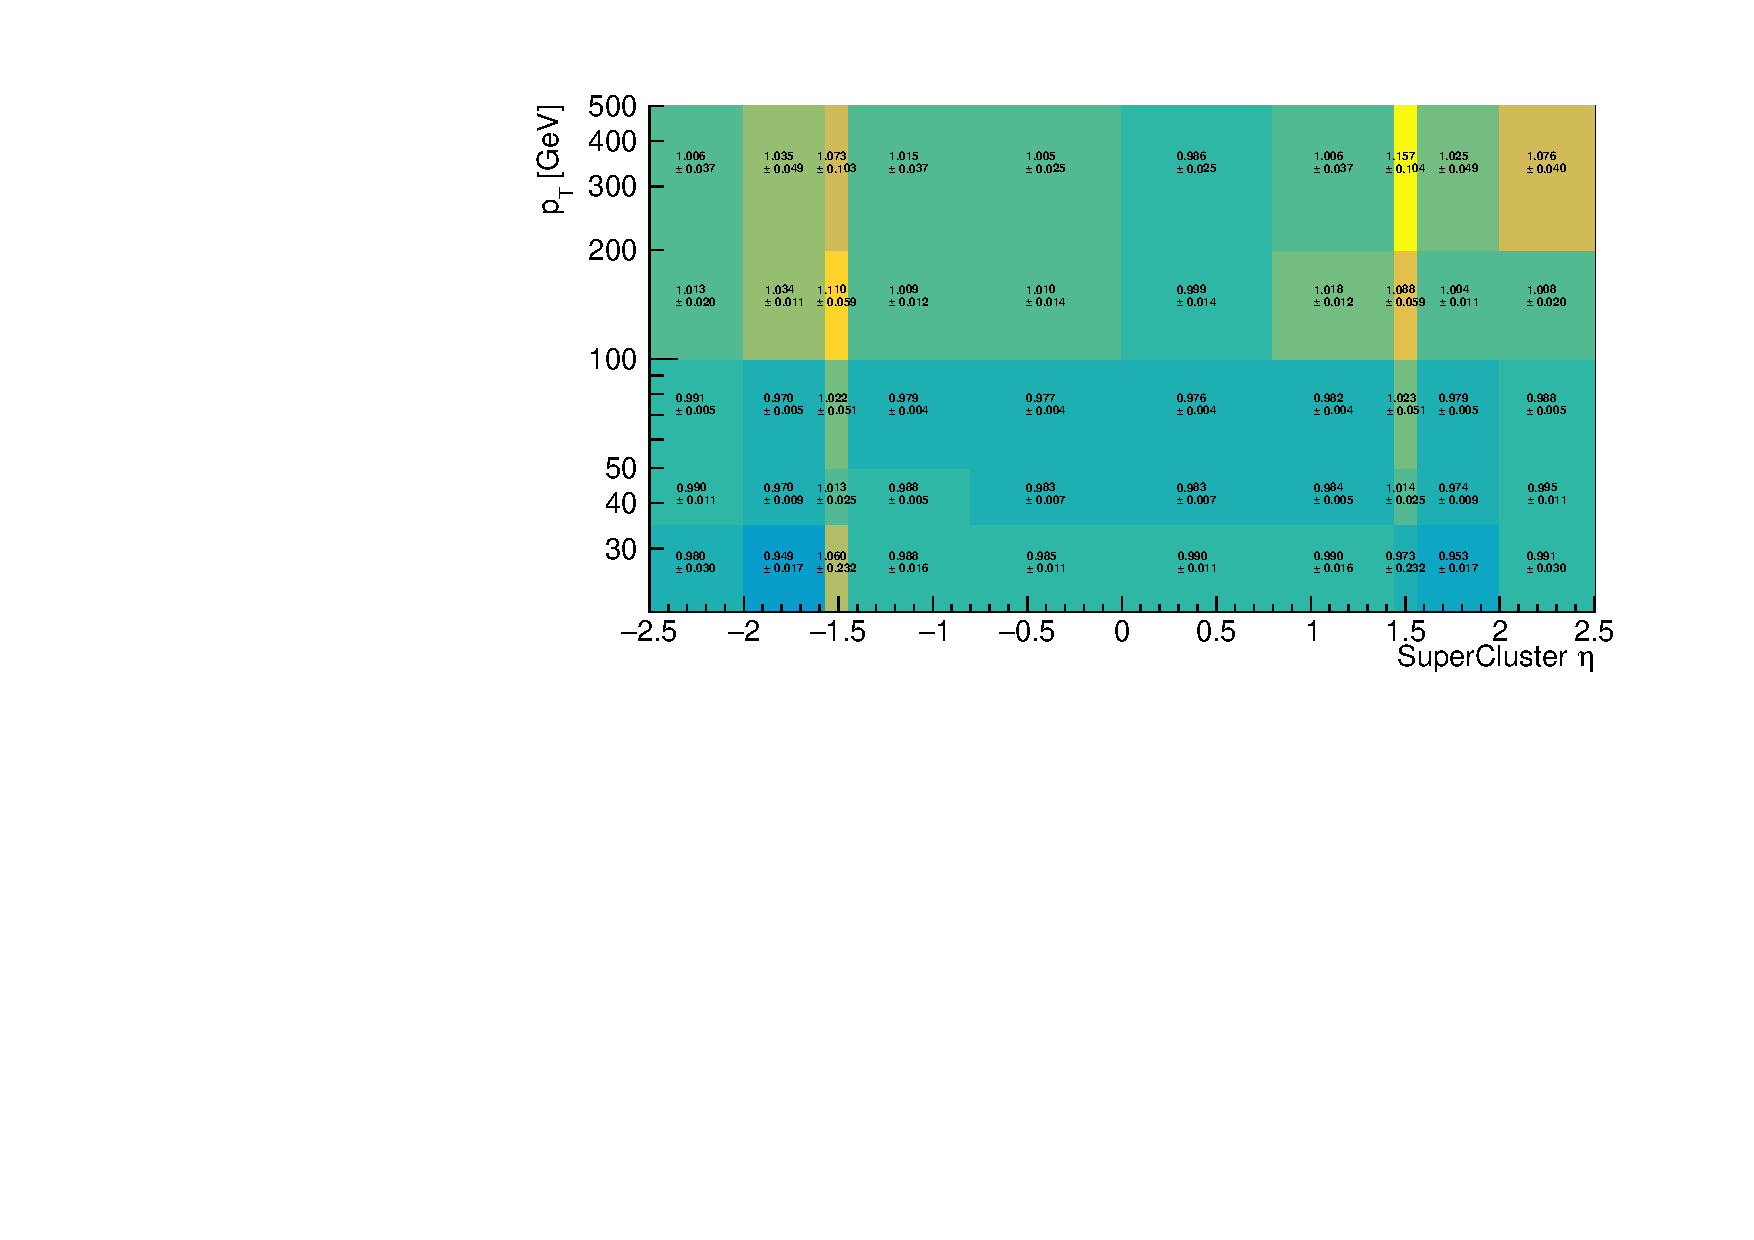
\includegraphics[width=.5\textwidth]{SF/phEffSF_2018.pdf}}}
  \caption{Photon efficiency scale factors for the cut-based Loose ID.}
  \label{fig:phEffSF}
\end{figure}

Besides the identification working points, an electron veto selection (CSEV veto) is also applied.
%% The scale factors are shown in ~\ref{tab:eleveto_SFs}.

%% \begin{table}[htbp]
%%  \centering
%%    \begin{tabular}{|c|c|l|l|}
%%    \hline
%%    Year & $p_T$& barrel & endcap\\ \hline
%%    2016 & inclusive &0.9938 $\pm$ 0.0119 & 0.9875 $\pm$ 0.0044\\\hline
%%    2017 & inclusive & 0.9862 $\pm$ 0.0030 & 0.9638 $\pm$ 0.0047\\\hline
%%    \multirow{3}{*}{2018} &10 GeV$<p_{T}^{\gamma}<30$ GeV &0.9869 $\pm$ 0.0043& 0.9535 $\pm$ 0.0054\\
%%    & 30 GeV$<p_{T}^{\gamma}<$60 GeV  &0.9908  $\pm$ 0.0111 & 0.9646 $\pm$ 0.0076\\
%%    & 60 GeV$<p_{T}^{\gamma}<$200 GeV &1.0084  $\pm$ 0.0856& 1.0218 $\pm$ 0.1178\\
%%    \hline
%%    \end{tabular}
%%    \caption{Electron veto scale factors for barrel and endcap corresponding to 2016 to 2018.}
%%    \label{tab:eleveto_SFs}
%%  \end{table}

%\begin{figure}[b]
%  \begin{center}
%    \includegraphics[width=0.8\textwidth]{figs/photon_SFs.pdf}
%    \caption{Photon ID scale factors for cut-based loose Photon selection}
%    \label{fig:PhotonEff}
%  \end{center}
%\end{figure}

\paragraph{Multivariate ID\\}
A more sophisticated photon identification strategy, is based on a multivariate technique, based on a Boosted Decision Tree (BDT) \cite{CMS:EGM-17-001}.
This multivariate (MVA) discriminant is built based on 14 input variables,
and provides excellent separation between signal (prompt photons) and background from misidentified jets.
The signal is defined as reconstructed photons from a \PGg + jets simulated sample that are matched at generator level with prompt photons within a cone of size $\DR = 0.1$,
whereas the background is defined by reconstructed photons in the same sample that do not match with a generated photon.
Photon candidates with $\ET > 15 \GeV$, $|\eta| < 2.5$, and satisfying very loose preselection requirements are used for the training of the BDT.
The variables used include the energy and shower shape of the supercluster, as well as various isolations.
Some of these variables are also employed by the cut-based ID, so the two discriminants are not independent.
%% The full list is shown in Table~\ref{tab:MVAvariables}.
%% The version used is \texttt{RunIIFall17v2}.

%% \begin{table}[ht]
%% \caption[.]{Variables used by the MVA-based ID, version \texttt{RunIIFall17v2}}
%% \label{tab:MVAvariables}
%% \centering
%% \begin{tabular}{l|l}
%% Name & variable\\
%% \hline
%% SCRawE             & superCluster.rawEnergy                                               \\
%% r9                 & r9                                                                   \\
%% sigmaIetaIeta      & full5x5\_showerShapeVariables.sigmaIetaIeta                          \\
%% etaWidth           & superCluster.etaWidth                                                \\
%% phiWidth           & superCluster.phiWidth                                                \\
%% covIEtaIPhi        & full5x5\_showerShapeVariables.sigmaIetaIphi                          \\
%% s4                 & full5x5\_showerShapeVariables.e2x2/full5x5\_showerShapeVariables.e5x5\\
%% scEta              & superCluster.eta                                                     \\
%% rho                & fixedGridRhoAll                                                      \\
%% esEffSigmaRR       & full5x5\_showerShapeVariables.effSigmaRR                             \\
%% esEnergyOverRawE   & superCluster.preshowerEnergy/superCluster.rawEnergy                  \\
%% phoIso03           & photonIso                                                            \\
%% chgIsoWrtChosenVtx & chargedHadronIso                                                     \\
%% chgIsoWrtWorstVtx  & chargedHadronWorstVtxIso                                             \\
%% \end{tabular}
%% \end{table}

Two working points are provided centrally by the the dedicated group within CMS:
\texttt{wp90} and \texttt{wp80}, corresponding to 90 \% and 80 \% prompt photon efficiency respectively.
The cuts on the MVA estimator value that define the two working points are detailed in Table~\ref{tab:MVAwpCuts}.

\begin{table}[ht]
\caption[.]{Working points of the photon MVA-based ID, version \texttt{RunIIFall17v2}}
\label{tab:MVAwpCuts}
\centering
\begin{tabular}{lrr}
\toprule
Name & Barrel & Endcap \\
\midrule
\texttt{wp80} & -0.02 & -0.26 \\
\texttt{wp90} &  0.42 &  0.14 \\
\bottomrule
\end{tabular}
\end{table}

As with any other ID, to account for difference in the modelling of its efficiency in simulations and the true efficiency in data,
Scale Factors are measured for each year in different bins of \pt and $\eta$ for \texttt{wp80} (Figure \ref{fig:phEffMVASF_wp80}) and \texttt{wp90} (Figure \ref{fig:phEffMVASF_wp90}).

\begin{figure}
\centering
\subfigure [2016preVFP ] {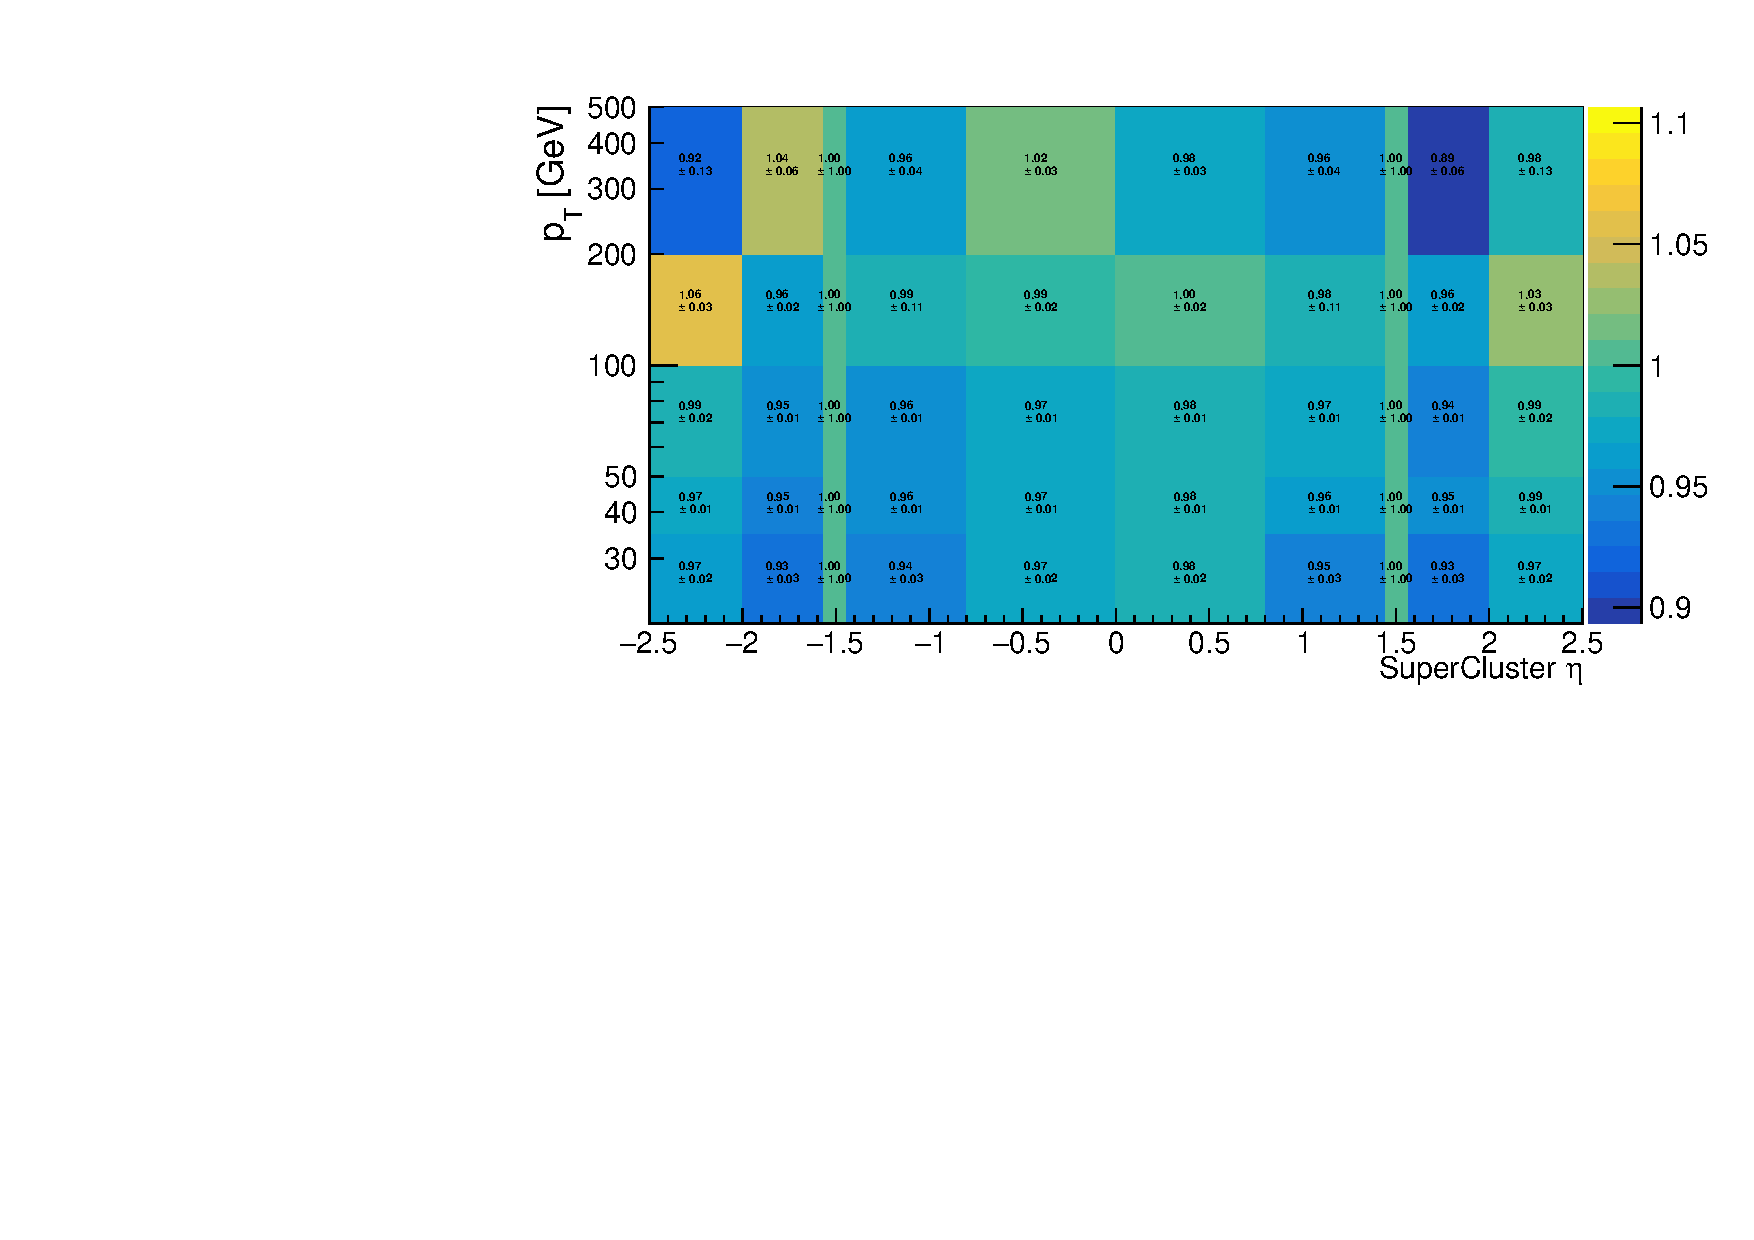
\includegraphics[width=.5\textwidth]{SF/2016_PhotonsMVAwp80_SF2D.pdf}}%
\subfigure [2017]        {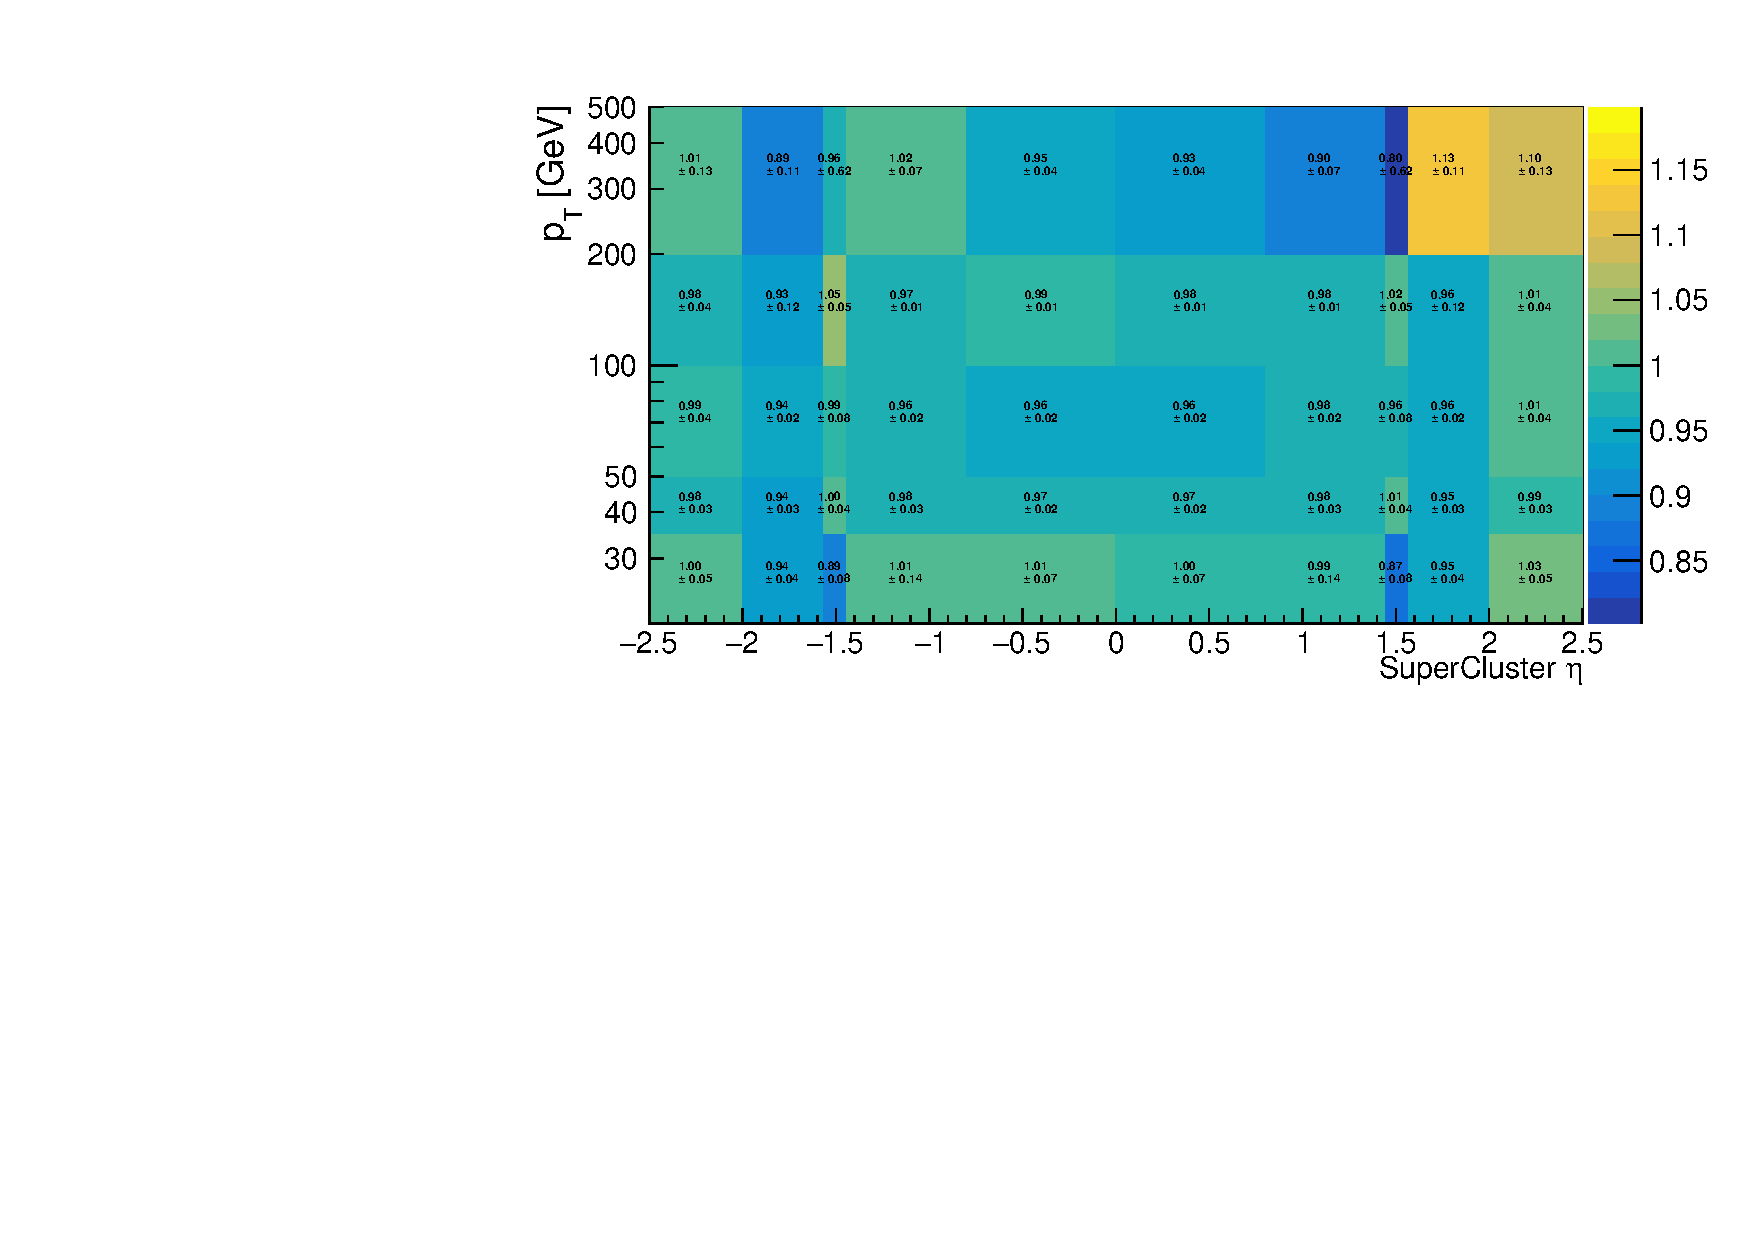
\includegraphics[width=.5\textwidth]{SF/2017_PhotonsMVAwp80_SF2D.pdf}}\\
\subfigure [2018]        {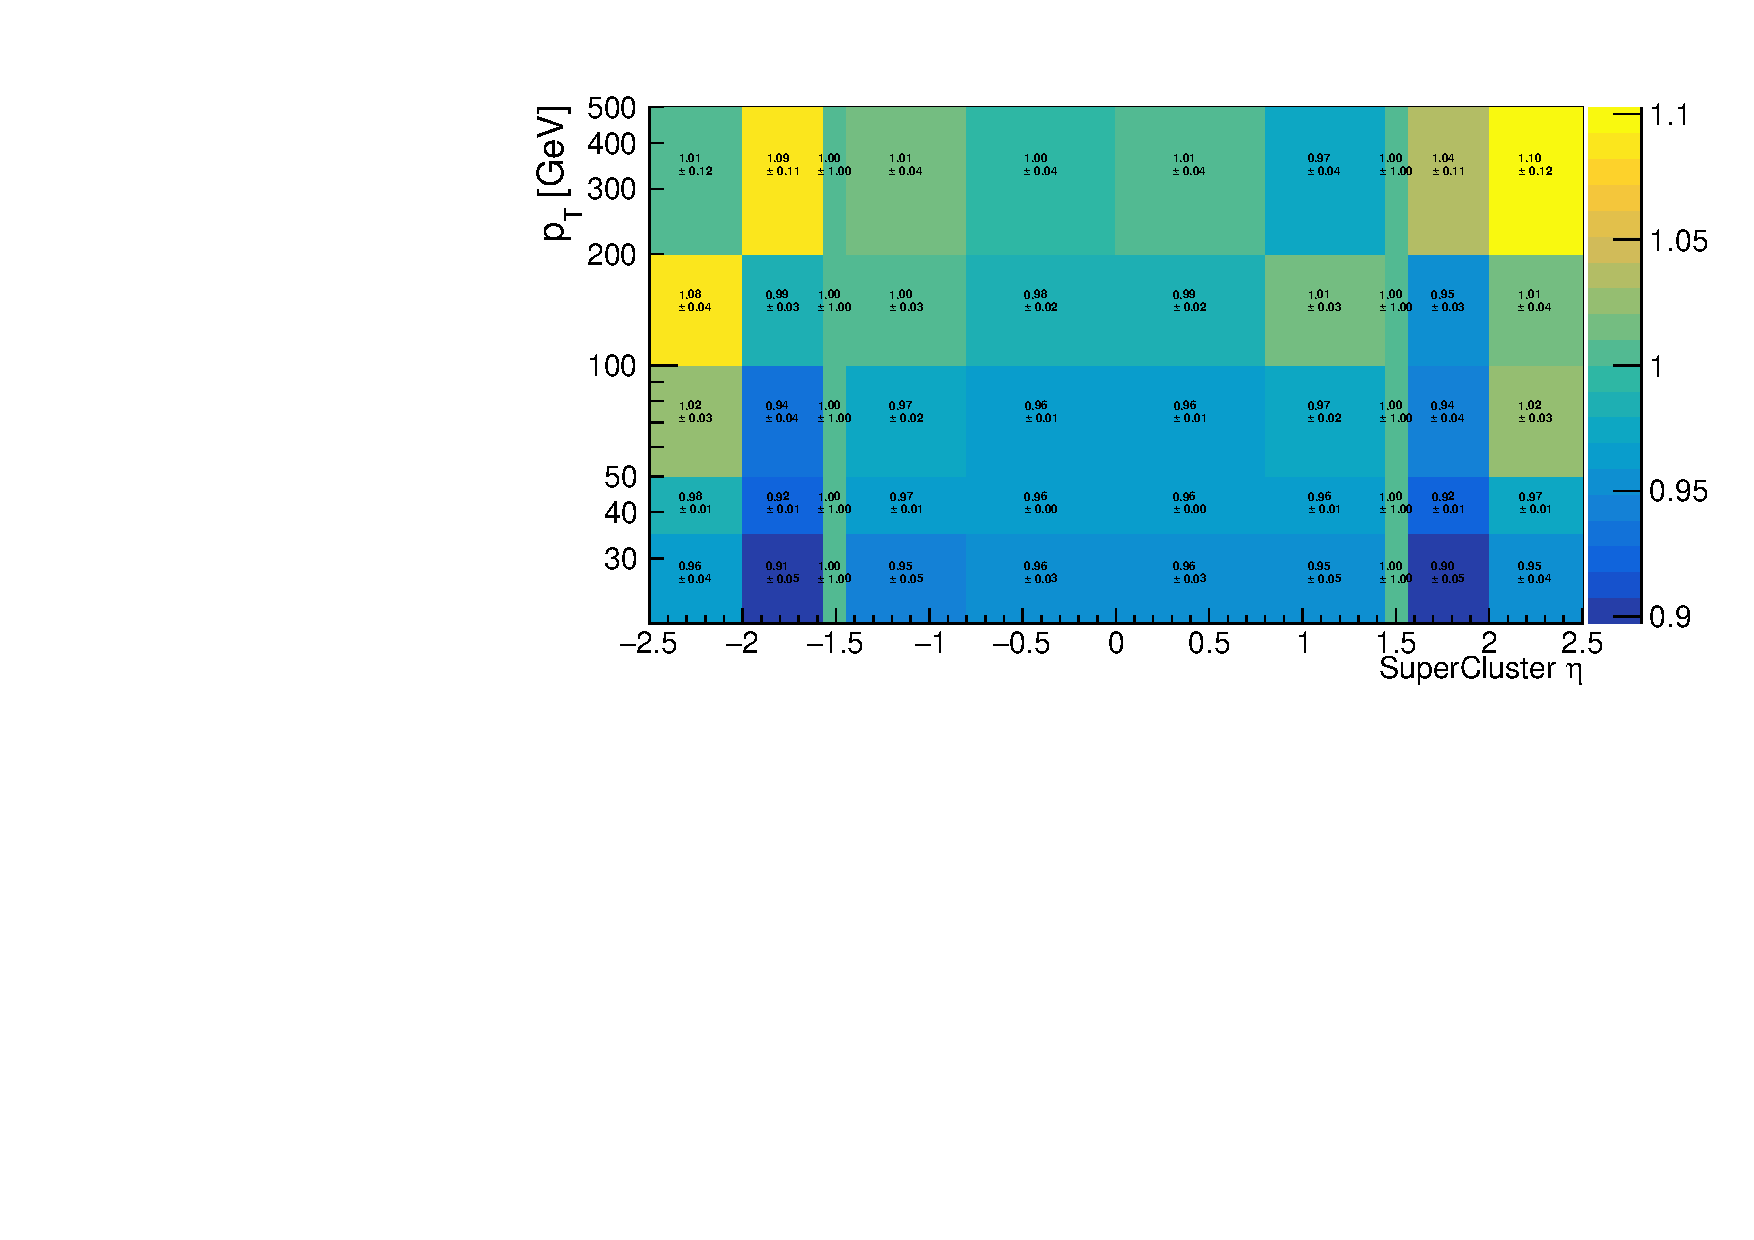
\includegraphics[width=.5\textwidth]{SF/2018_PhotonsMVAwp80_SF2D.pdf}}
\caption{Photon efficiency scale factors for the MVA-based ID with working point \texttt{wp80}.}
\label{fig:phEffMVASF_wp80}
%% }
\end{figure}

\begin{figure}
\centering
\subfigure [2016preVFP ] {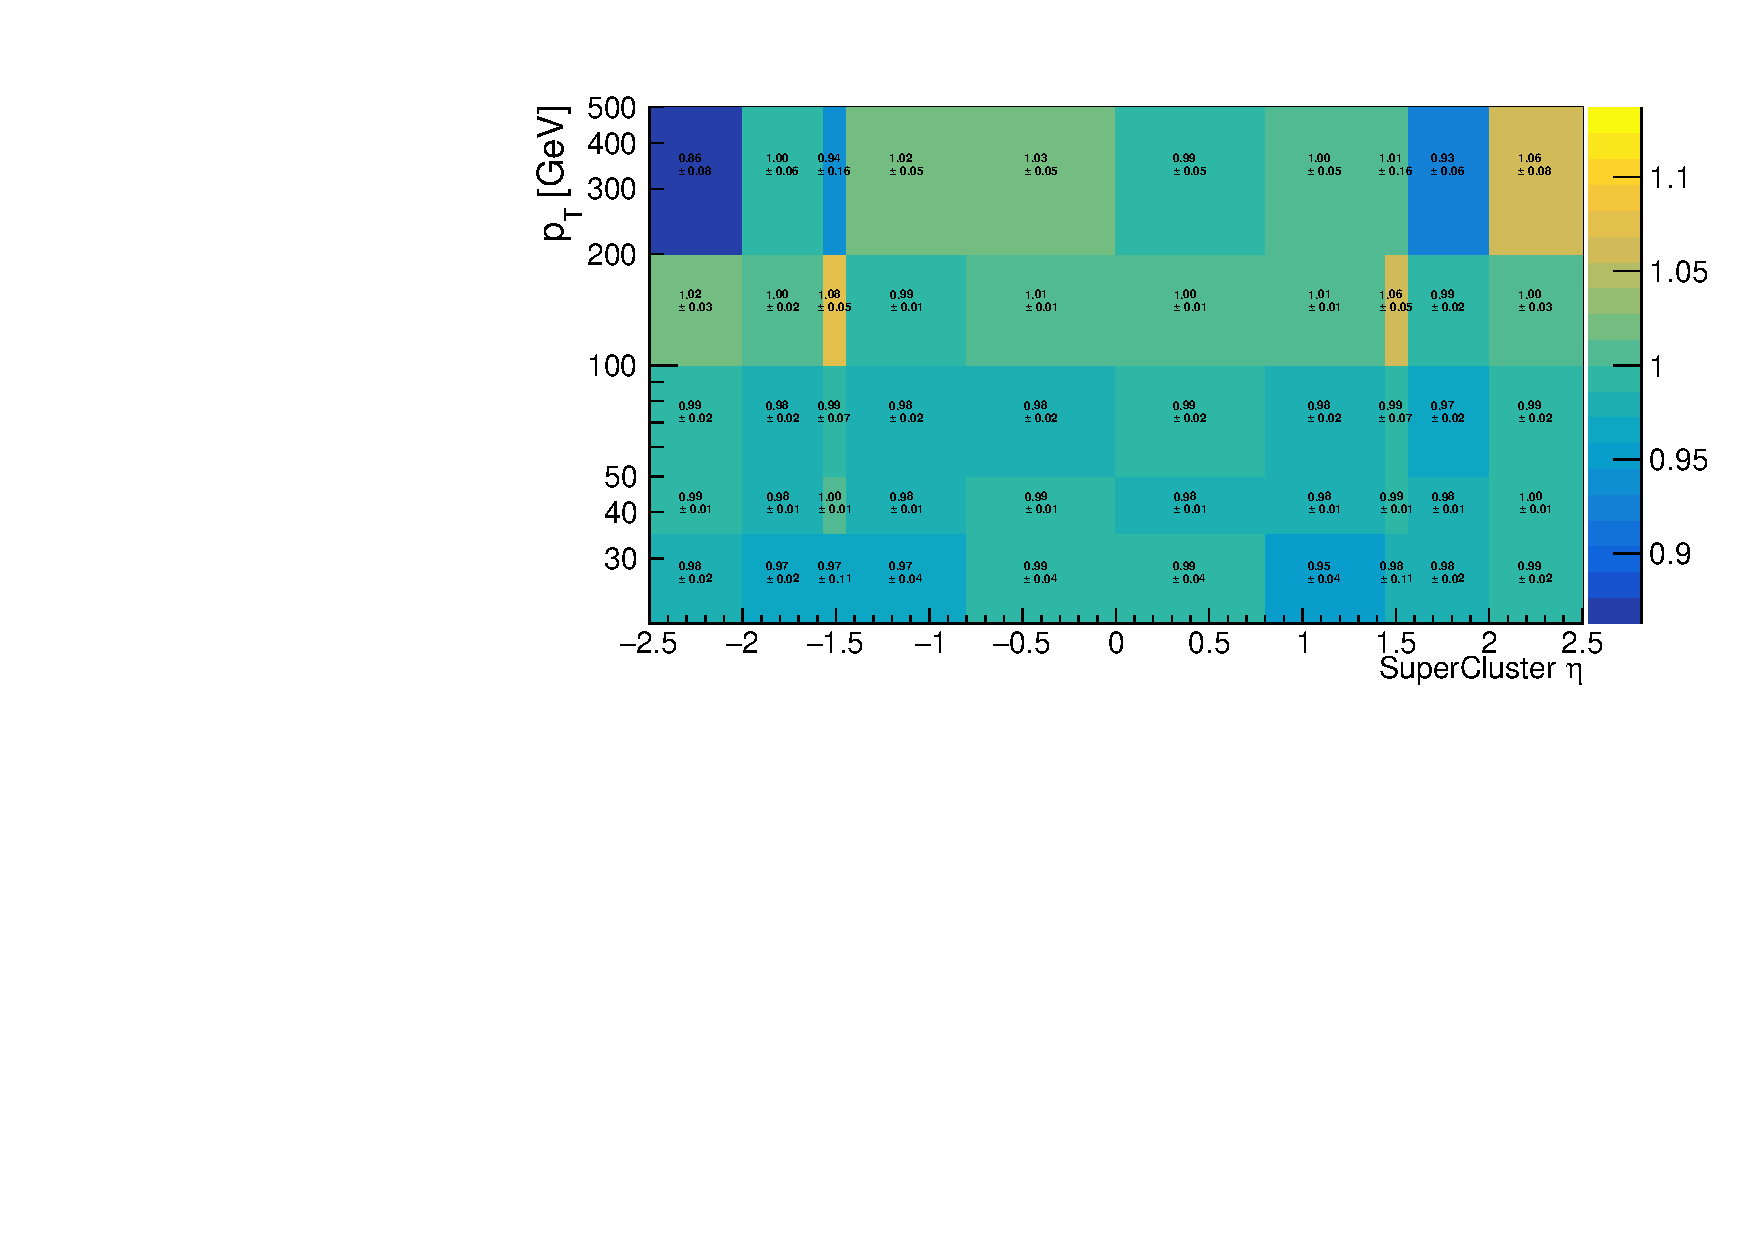
\includegraphics[width=.5\textwidth]{SF/2016_PhotonsMVAwp90_SF2D.pdf}}%
\subfigure [2017]        {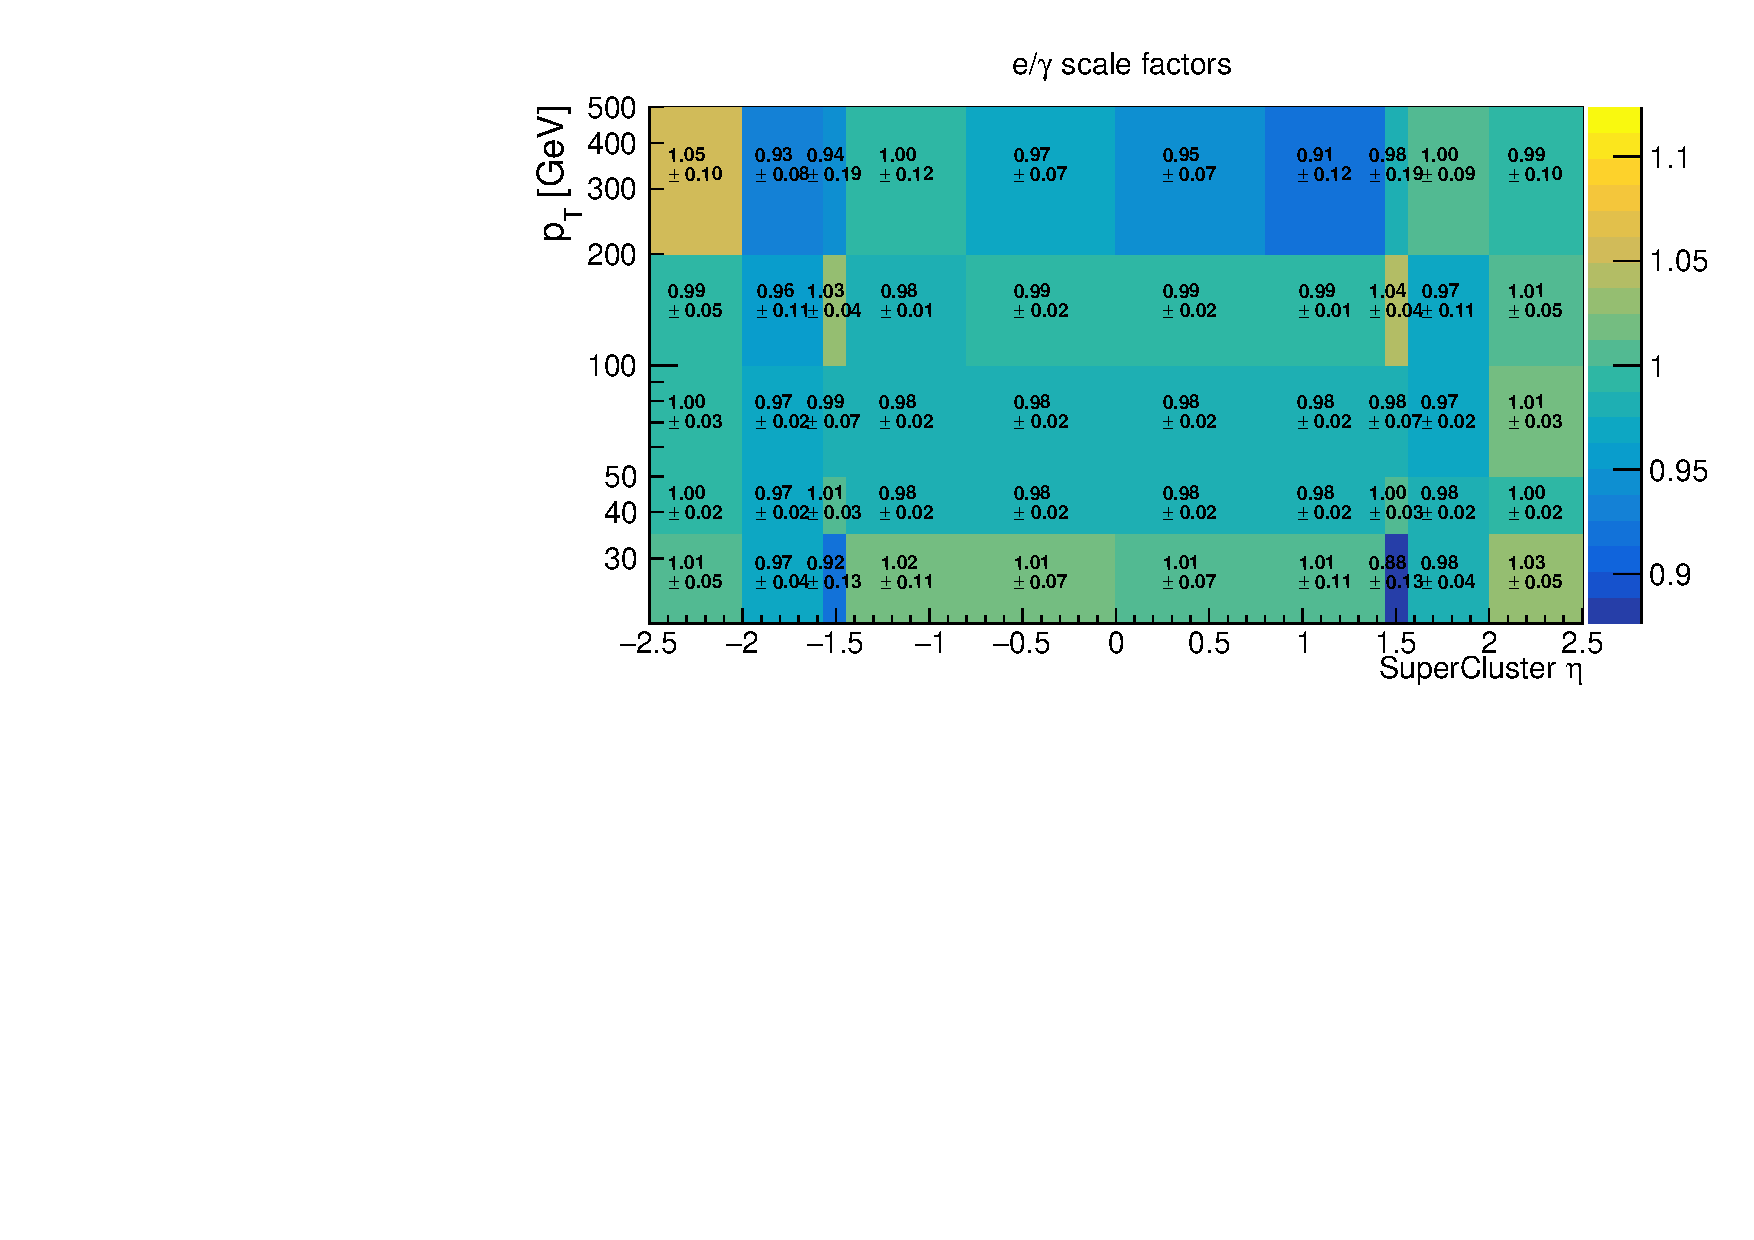
\includegraphics[width=.5\textwidth]{SF/2017_PhotonsMVAwp90_SF2D.pdf}}\\
\subfigure [2018]        {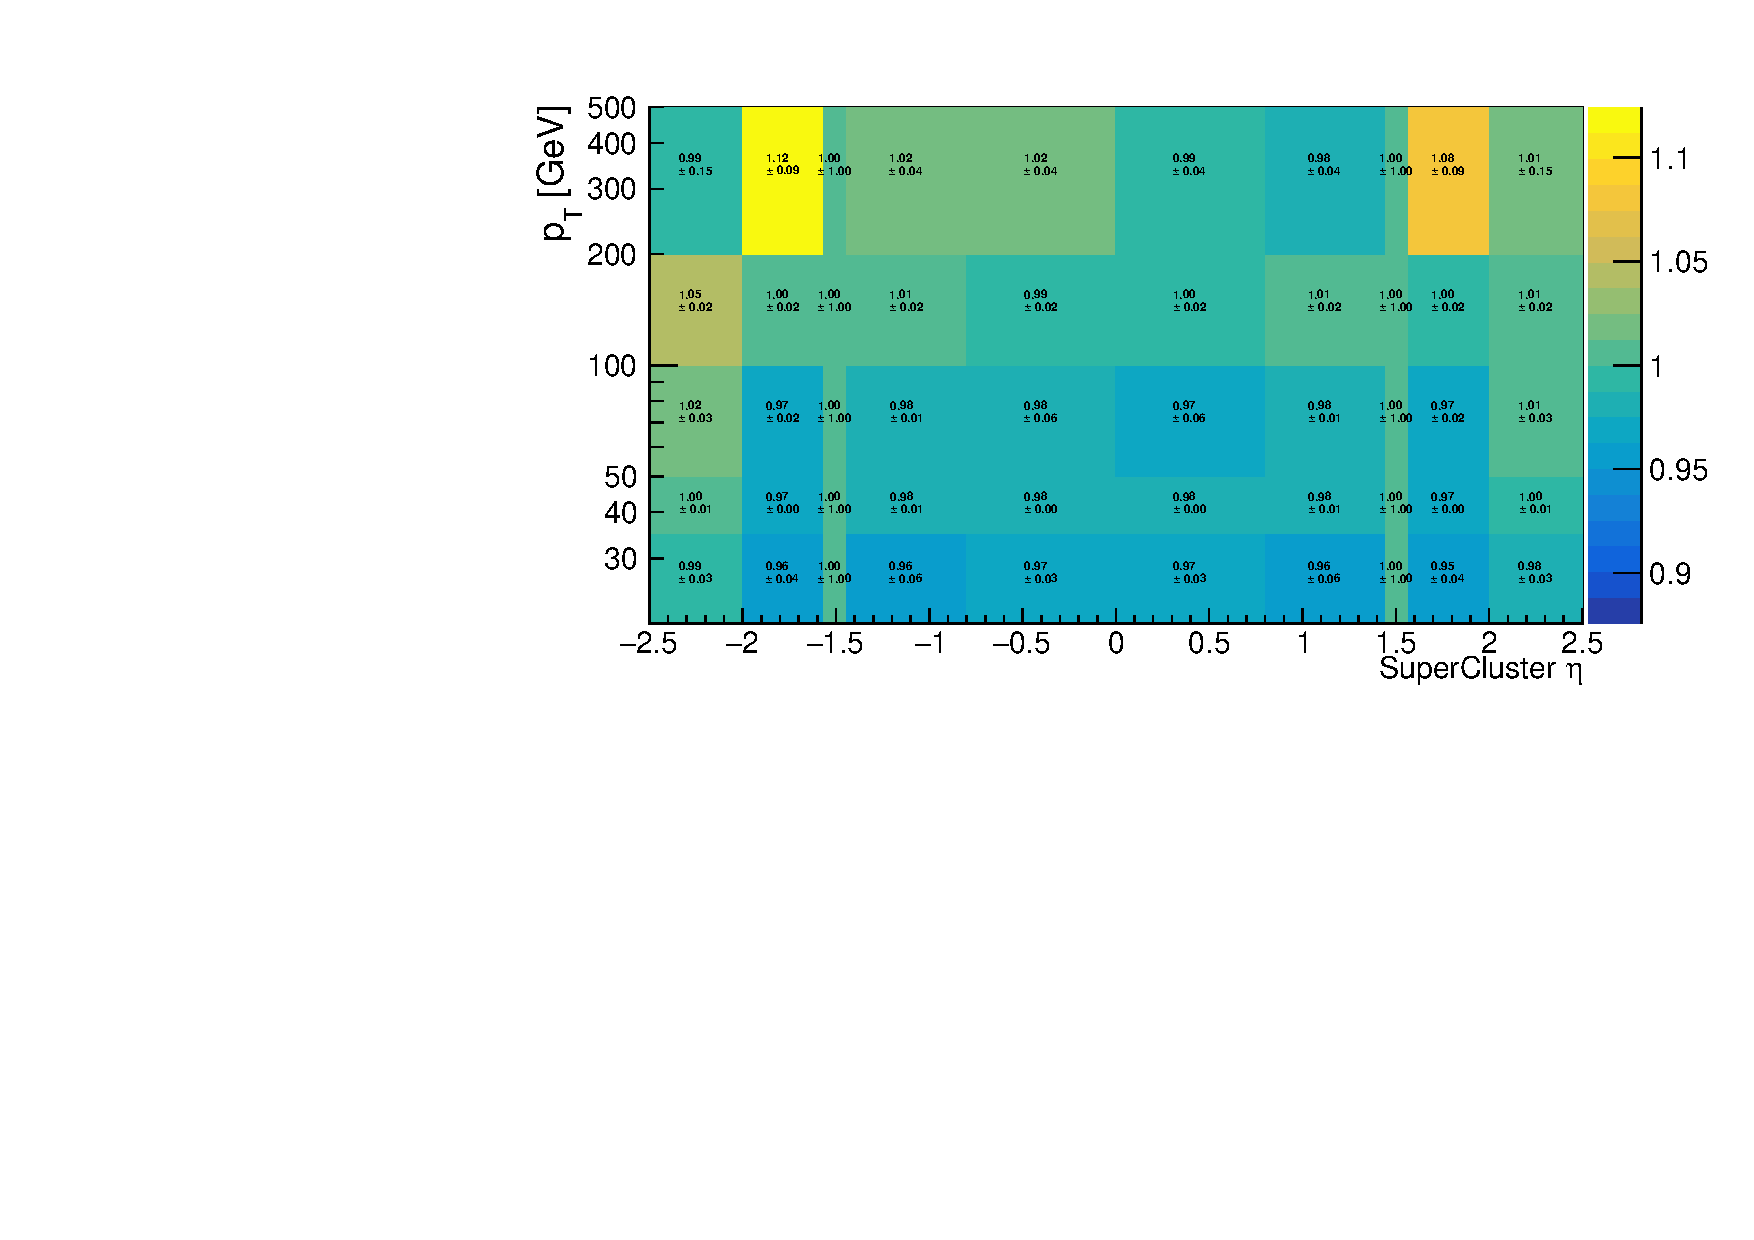
\includegraphics[width=.5\textwidth]{SF/2018_PhotonsMVAwp90_SF2D.pdf}}
\caption{Photon efficiency scale factors for the MVA-based ID with working point \texttt{wp90}.}
\label{fig:phEffMVASF_wp90}
\end{figure}

A comparison between the cut-based and the MVA-based IDs is shown in Figure~\ref{fig:PhotonIsoAUC}.
It represent the background rejection as a function of the signal efficiency for the raw MVA discriminant
and the three working points of the cut-based ID.

\begin{figure}
\centering
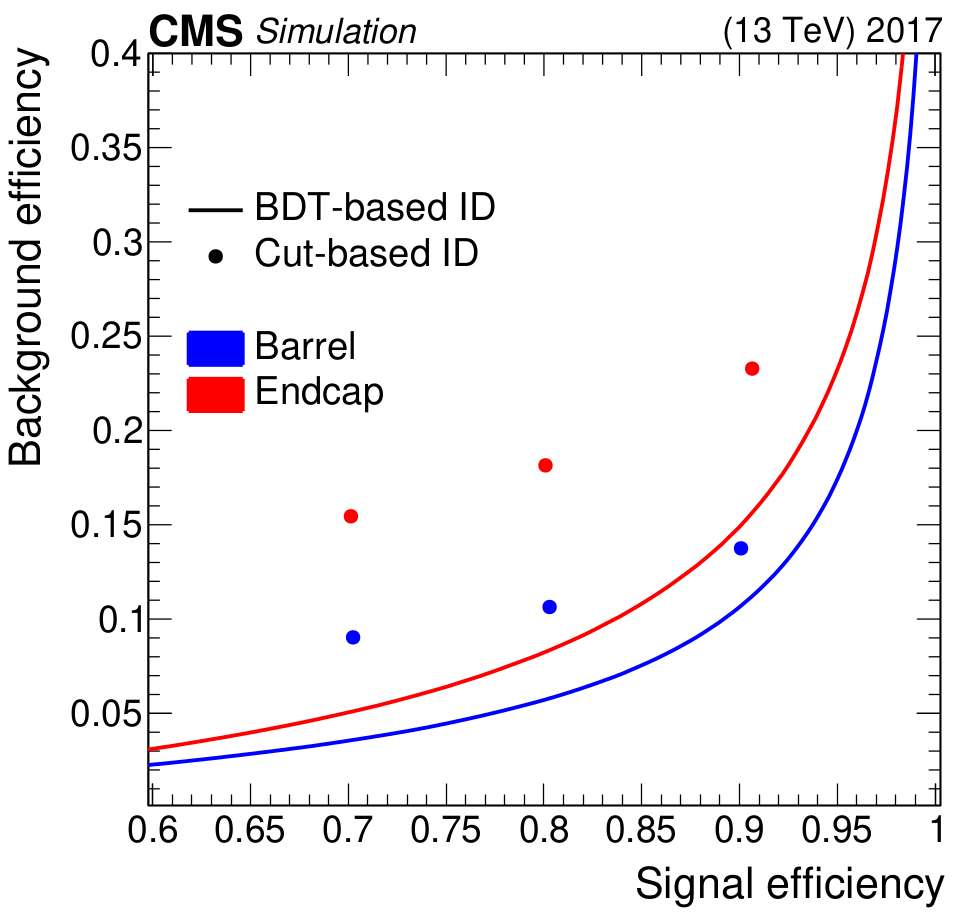
\includegraphics[width=.5\textwidth]{PhotonIsoAUC.png}
\caption{Performance of the photon BDT and cut-based identification algorithms in 2017.
Three different working points (loose, medium and tight) are shown for the cut-based ID. \cite{CMS:photon-performance-2015}}
\label{fig:PhotonIsoAUC}
\end{figure}

\paragraph{Selections used in the analysis\\}
\label{sec:photon_selection}

A common base selection is applied to all the photons, consisting of
\pt > 20 \GeV and
$|\eta| < 1.4442$ OR $1.566 < |\eta| < 2.4$.
Photons must also pass a conversion safe electron veto (CSEV) \cite{CMS:photon-performance-2015} which requires the absence of charged particle tracks,
with a hit in the innermost layer of the pixel detector not matched to a reconstructed conversion vertex, pointing to the photon cluster in the ECAL.
Photons are also rejected in the presence of a seed in the pixel tracker consisting of at least two hits,
which points to the ECAL within some window defined around the photon SC position.
Photons that pass these selections are called \textbf{kinematic photons}, which is the loosest selection used in this analysis.

Photons that also pass the cut thresholds of the Loose cut-based ID (see Table~\ref{tab:VPhotonID}) for H/E, the neutral ($I_n$) and photon ($I_\PGg$) isolations
are defined \textbf{very loose} photons.
They are used as the loose working point in a tight-to-loose method (Section \ref{sec:fake_photons_background}) to estimate the \nonprompt photon background.

The photons that also pass the \sieie and charged isolation ($I_{ch}$), and thus the Loose cut-based ID, are the \textbf{loose photons},
which is the tight selection for the \nonprompt photon background,
and the analysis selection for the results derived using the cut-based ID.

Additionally, kinematic photons that pass the MVA-based working points wp90 and wp80 are also considered,
given the improved performance of the MVA ID over the cut-based one.
The drawback of this ID is that it is not possible to do a data-driven estimation of the \nonprompt background,
due to the limited size of the application region defined by requiring a photon that passes the wp90 but fails the wp80,
as explained in Section~\ref{sec:fake_photons_background}.


\subsection{Jets}
\subsubsection{Jet Identification}
\label{sec:jet_ID}
In order to assure a good reconstruction efficiency, identification quality criteria are imposed on jets based on
the energy fraction of the charged, electromagnetic, and neutral hadronic components \cite{CMS-PAS-JME-16-003}.

To reduce instrumental background, the jet identification criteria described in Table \ref{tab:JetID2018} is used.

\begin{table}
  \caption{Jet identification criteria used in \RunII{} with thresholds used for 2018 data.}
  \label{tab:JetID2018}
  \resizebox{\textwidth}{!}{
  \begin{tabular}{l c c c c}
    \toprule
    Variable                    & $|\eta| \le 2.6$ & $2.6 < |\eta| \le 2.7$ & $2.7 < |\eta| \le 3.0$ & $3.0 < |\eta| \le 5.0$\\
    \midrule
    Neutral Hadron Fraction     & < 0.90           & < 0.90                 & -                      & > 0.2                 \\
    Neutral EM Fraction         & < 0.90           & < 0.99                 & $<0.99\ \land\,>0.02$  & < 0.9                 \\
    Number of Constituents      & > 1              & -                      & -                      & -                     \\
    Muon Fraction               & < 0.80           & < 0.80                 & -                      & -                     \\
    Charged Hadron Fraction     & > 0              & -                      & -                      & -                     \\
    Charged Multiplicity        & > 0              & > 0                    & -                      & -                     \\
    Charged EM Fraction         & < 0.80           & < 0.80                 & -                      & -                     \\
    Number of Neutral Particles & -                & -                      & > 2                    & > 10                  \\
    \bottomrule
  \end{tabular}
  }
\end{table}

In this analysis, the jets are required to be within $|\eta| < 4.7$ and to have a transverse momentum above 30\GeV.

The identification of jets originated by the hadronization of heavy-flavour quarks is achieved through the DeepFlavour tagger \cite{Guest_2016, CMS-BTV-16-002}.
It uses a deep neural network with input variables from up to six tracks from each jet, information on secondary vertices and on the jet itself,
such as the energy and total number of tracks.
It assigns five probabilities to each jet, namely to contain only one \PQb hadron, two or more \PQb hadrons, exactly one \PQc hadron, at least two \PQc and no \PQb hadrons, or none of the above.
In the two and three lepton channels there is the need to exclude events containing top quarks,
since their decay $\PQt \to [\PW \to \Pl\PGn] \PQb$ produces additional charged leptons which may lower the purity of the signal regions.
Thus the need to identify jets induced by the hadronization of \PQb quarks,
which is achieved by summing the probabilities of the first two categories,
which are the single b hadron and the two or more b hadrons.
Working points are defined for this ID, as shown in Table \ref{tab:DeepFlavourBtagWP}.

\begin{table}
  \caption{Working points of the combined b-tag with the DeepFlavour classifier and the corresponding misidentification probability.}
  \label{tab:DeepFlavourBtagWP}
  \centering
  \begin{tabular}{l c c}
    \toprule
    \makecell{Working\\point} & Threshold & \makecell{Misidentification\\probability}\\
    \midrule
    Loose  & 0.0494 & 10  \%\\
    Medium & 0.2770 & 1   \%\\
    Tight  & 0.7264 & 0.1 \%\\
    \bottomrule
  \end{tabular}
\end{table}

In addition this analysis considers also a collection of \textbf{large radius jets} clustered using the same \antikt algorithm with a distance parameter $R = 0.8$.
These jets are cleaned using the Pileup Per Particle Identification (PUPPI) \cite{Bertolini_2014}, which is a method for \pileup{} mitigation.

\paragraph{Jet disambiguation\\}
The PF jet collection contains jets clustered with \antikt on all the particles reconstructed from Particle Flow.
This means that isolated and energetic leptons and photons, which are part of the signal definition,
are likely to be in the core of a jet due to the nature of the algorithm.
Therefore a disambiguation strategy is needed to avoid double counting entities.
Jets are removed if they match any of the leptons passing the Loose ID
and photons, either FSR associated to a lepton or candidates passing the kinematic selection (Section \ref{sec:photonID}),
by requiring: $\DR(\text{jet,\,lepton/photon}) > 0.4$.


\subsection{Summary}
The requirements on all objects used for the analysis with 2016, 2017 or 2018 data are summarized in the Table~\ref{tab:objsummary}. In addition, a ``ghost-cleaning'' procedure is applied to the muons, as described in Sec.~\ref{sec:muonReco}. 

A lepton is declared {\bf loose} if it passes the reconstruction, kinematics and dxy/dz cuts and declared {\bf tight} if it passes in addition the identification, isolation and SIP3D requirements. 

\begin{table}
  \centering
  \caption{Summary of physics object selection for the analysis.}
  \label{tab:objsummary}
  %% \resizebox{\textwidth}{!}{
    \begin{tabular}{l l}
      \toprule
      \multirow{4}{*}{Electrons}
        & $\pt^e > 7 \GeV$   \quad $\abs{\eta^e} < 2.5$ \\
        & $d_{xy} < 0.5 \cm$ \quad $d_{z} < 1 \cm$      \\
        & $\SIPthreeD < 4$                              \\
        & MVA ID with isolation cuts from Section~\ref{sec:eleMVA}\\
      \midrule
      \multirow{5}{*}{Muons}
        & Global or Tracker Muon                                 \\
        %% & Discard muons with muonBestTrackType==2 even if they are global or tracker muons \\
        & $\pt^{\mu} > 5 \GeV$ \quad $\abs{\eta^{\mu}} < 2.4$    \\
        & $d_{xy} < 0.5 \cm$   \quad $d_{z} < 1 \cm$             \\
        & $\SIPthreeD < 4$                                       \\
        & BDT with ID, isolation from Section~\ref{sec:muo_selection}\\
      \midrule
      \multirow{4}{*}{FSR photons}
        & $\pt^{\PGg} > 2 \GeV$ \quad $\abs{\eta^{\PGg}} < 2.4$     \\
        & ${\cal I}_{\mathrm{PF}}^{\PGg} < 1.8$                     \\
        & $\DR(\ell,\,\PGg) < 0.5$                                  \\
        & $\frac{\DR(\Pl,\,\PGg)}{(\pt^{\PGg})^2} < 0.012 \GeV^{-2}$\\
        \noalign{\vspace{.3ex}} % small vertical space
      \midrule
      \multirow{5}{*}{Signal photons}
        & $\pt^{\PGg} > 20 \GeV$                        \\
        & $\abs{\eta^{\PGg}} < 2.4 \; \land \abs{\eta^{\PGg}} \notin (1.4442, 1.566) $\\
        & $\DR(\ell,\,\PGg) > 0.5$                      \\
        & Conversion Safe Electron Veto                 \\
        & Cut-based (Loose wp) or MVA (wp90 or wp80) ID \\
      \midrule
      \multirow{5}{*}{Jets}
        & $\pt^{\mathrm{jet}} > 30 \GeV$ \quad $\abs{\eta^{\mathrm{jet}}} < 4.7$ \\
        & $\DR(\ell/\PGg,\, \mathrm{jet}) > 0.4$    \\
        & Cut-based jet ID (tight WP)               \\
        & Jet \pileup{} ID (tight WP)               \\
        & Deep CSV b-tagging (medium WP)            \\
      \bottomrule
    \end{tabular}
  %% }
\end{table}


\section{Calibration and efficiency measuremtents}
\note{Maybe move to next chapter}
\subsection{Electrons}
\subsubsection{Electron Energy Calibrations}
%\textbf{FIXME: ReRecoed data are used but additional e-scale and smearing corrections NOT yet available and thus NOT yet applied}
Electrons in data are corrected for features in ECAL energy scale
in bins of $\pt$ and $\left| \eta \right|$. Corrections are calculated
on a $\cPZ \to \Pe\Pe$ sample to align the dielectron   
mass spectrum in the data to that in the MC, and to
minimize its width.

The $\cPZ \to \Pe\Pe$ mass resolution in Monte Carlo is made to match
data by applying a pseudo-random Gaussian smearing to electron energies,
with Gaussian parameters varying in bins of $\pt$ and $\left| \eta \right|$.
This has the effect of convoluting the electron energy spectrum with a
Gaussian.

The electron energy scale is measured in data by fitting a Crystal-ball function to the di-electron mass spectrum around the Z peak in the $Z\rightarrow \Pe \Pe$ control region.
% The energy scale for the 2016, 2017 and 2018 dataset are shown in Fig.~\ref{fig:ele_energy_scaleA},~\ref{fig:ele_energy_scaleB},~\ref{fig:ele_energy_scaleC} (a), respectively, and decently agrees with the MC with the preliminary corrections released so far by EGAMMA POG. % for Moriond. % even without any corrections available at the moment. 


\subsubsection{Electron Efficiency Measurements}
\label{sec:eleEffMeas}
Electron efficiencies are evaluated using the Tag-and-Probe method~\cite{CMS-EWK-10-005}.
The study was performed on the SingleElectron/EGamma dataset for each year separately.

Tag electrons need to satisfy the following quality requirements:
\begin{itemize}
\item trigger matched to single electron trigger;
\item $\pt > 30 \GeV$, supercluster (SC) $|\eta| < 2.17$;% but on in EB-EE gap ($1.4442<|\eta|<1.566$)
\item the tag and the probe need to have opposite charge.
%\item tight working point of the Spring16 cut-based electron ID
\end{itemize}

For the bin of probe \pt between 7 and 20\GeV, additional criteria are required:
\begin{itemize}
\item the tag has to pass a cut on the MVA score;
\item $\sqrt{2*\ptmiss*\pt^{tag}*(1-cos(\phi_{\rm MET}-\phi_{tag}))} < 45 \GeV$;
\item tag minimum \pt increased to 50\GeV;
\item the charge is determined with the so-called selection method, requiring that all three estimates of the electron charge to agree.
\end{itemize}
These cuts help cleaning the background and make the fits more reliable (and thus, the measurement more precise).

Probe electrons only need to be reconstructed with the Gaussian sum filter, while the FSR recovery algorithm is not applied.

The nominal simulation efficiencies are evaluated from the a Drell-Yan sample simulated with \MADGRAPH at Leading Order in QCD,
using a template fit.
The $m_{ee}$ signal shape of the passing and failing probes are taken from MC and convoluted with a Gaussian.
The data is then fitted with the convoluted MC templates and a CMSShape (an Error-function with a one-sided exponential tail).
For the low \pt bins, a Gaussian is added to the signal model for the failing probes.

%\paragraph{Electron selection efficiency measurements}\mbox{}\\
%\label{par:Efficiency_measurements}

The electron selection efficiency is measured as a function of the probe electron $p_{T}$ and its SC $\eta$, and separately for electrons falling in the ECAL gaps.

%Figure \ref{fig:ele_sel_pt_turn_onA},~\ref{fig:ele_sel_pt_turn_onB},~\ref{fig:ele_sel_pt_turn_onC} and~\ref{fig:ele_ele_eta_turn_onA},\ref{fig:ele_ele_eta_turn_onB},~\ref{fig:ele_ele_eta_turn_onC} show the $p_{T}$ and $\eta$ turn-on curves measured in data, for 2016, 2017 and 2018.
% and the final 2D scale factor is shown in Fig.~\ref{fig:ele_sel_scale_factors} together with the systematic uncertainties. %These scale factors are very similar to the ICHEP figures, but more homogenous across $\eta$ and $p_{T}$ because of the higher statistics and the usage of more stable fitting routines in the new T\&P tool.

%\includegraphics[page=2, width=0.4\textwidth]{Figures/Electrons/ErecoEta}\\

Standard practices for the evaluation of Tag-and-Probe uncertainties for efficiency measurements are followed. Specifically, the following were considered:

\begin{itemize}
   \item Variation of the signal shape from the MC shape to an analytic shape (Crystal Ball) fitted to the MC
   \item Variation of the background shape from a CMS-shape to a simple exponential in fits to data
   \item Using an NLO MC sample for the signal templates
\end{itemize}

The total uncertainty for the measurement of the scale factors is the quadratic sum of the statistical uncertainties returned from the fit and the aforementioned systematic uncertainties.

The resulting efficiencies and corresponding scale factors, expressed as ratio of the efficiency observed in data to that calculated in simulation are reported
in Figure~\ref{fig:eleMVAEffSF}.

\begin{figure}
\centering
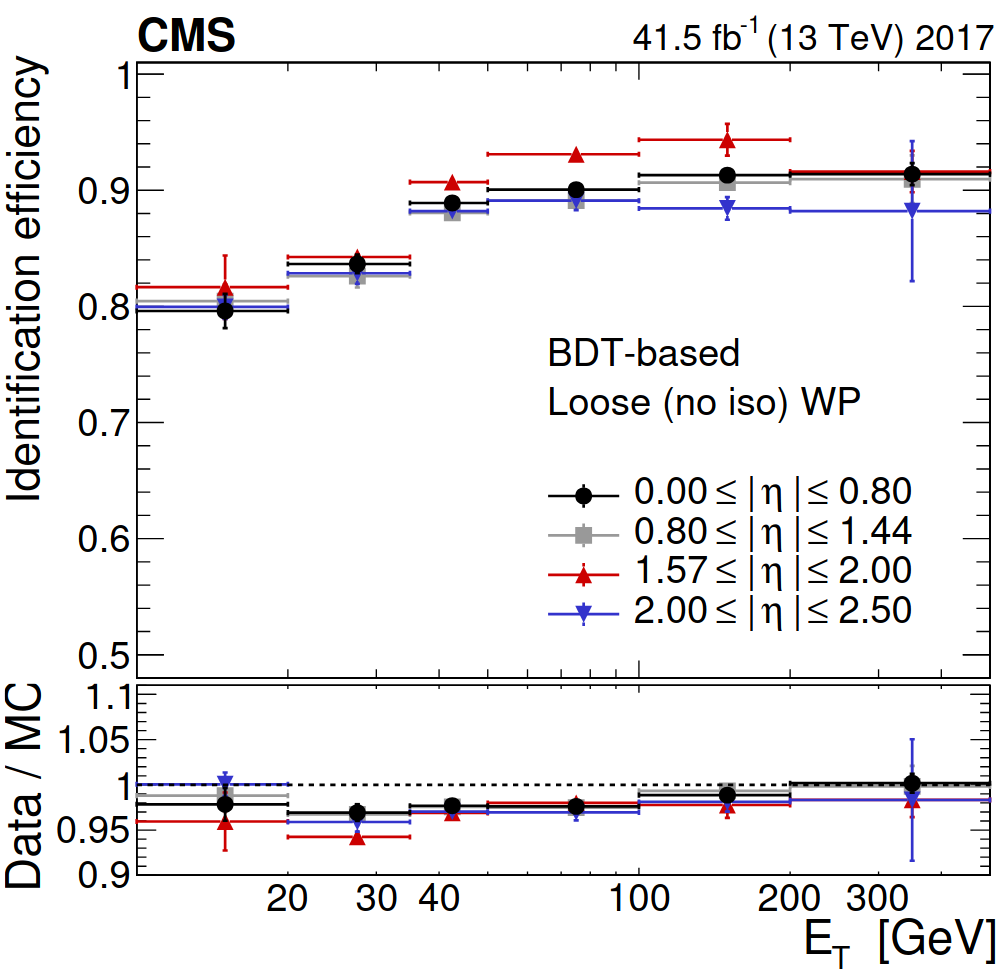
\includegraphics[width=.5\textwidth]{eleMVAEffSF2017.png}
\caption{Electron selection efficiencies in data (upper panel)
  and data-to-simulation ratio (lower panel),
  measured using the Tag-and-Probe technique
  as a function of the transverse energy}
\label{fig:eleMVAEffSF}
\end{figure}



\subsection{Muons}
\subsubsection{Muon Energy Calibrations}
\note{Remove, maybe?}
Similar to electrons the muon momentum scale is measured in data by fitting a Crystal-ball function to the di-muon mass spectrum around the Z peak in the 
$Z \rightarrow \mu\mu$ control region.
%At the moment no muon scale and resolution corrections are available but from 
%Fig.~\ref{fig:mu_energy_scaleA},~\ref{fig:mu_energy_scaleB} and~\ref{fig:mu_energy_scaleC} shows a very good agreement between data and simulation, for 2016, 2017 and 2018 eras, respectively. %even without any corrections.



\subsubsection{Muon Efficiency Measurements}
\note{Remove, maybe?}
\label{sec:muonEffMeas}
Muon efficiencies are measured with the Tag and Probe (T\&P) method performed on
$\cPZ \to \Pgm\Pgm$ and $\JPsi\to\mu\mu$ events in bins of $\pt$ and $\eta$. 
% More
%details on the methodology can be found in Ref.~\cite{CMS_AN_2015-277}. Measurements are extracted using 2018 RunA,B,C,D data while the measurements corresponding to 2016 and 2017 datasets have already been reported in Ref.~\cite{CMS_AN_2016-442} and Ref.~\cite{CMS_AN_2017-342} respectively.
%
The $\Z$ sample is used to measure the muon reconstruction and identification efficiency at high $\pt$,
and the efficiency of the isolation and impact parameter requirements at all $\pt$.
%
The $\JPsi$ sample is used to measure the reconstruction efficiency at low $\pt$,
as it benefits from a better purity in that kinematic regime. In this case,
events are collected using \verb=HLT_Mu7p5_Track2_Jpsi_v*= when probing the
reconstruction and identification efficiency in the muon system, and using the
 \verb=HLT_Mu7p5_L2Mu2_Jpsi_v*= when probing the tracking efficiency.

Results for the muon reconstruction and identification efficiency for $\pt > 20\GeV$
have been derived by the Muon POG.
The probe in this measurement are tracks reconstructed in the inner tracker, and
the passing probes are those that are also reconstructed as a global or tracker muon 
and passing the Muon POG Loose muon identification.
%
Results for low \pt muons were derived using \JPsi events, with the same definitions
of probe and passing probes. The systematic uncertainties are estimated by varying the analytical signal and background shape models used to fit 
the dimuon invariant mass. 
% Details on the procedure can be found in Ref.~\cite{AN-15-277}. 
The efficiency and scale 
factors used for low $\pt$ muons are the ones derived using single muon dataset.


For the impact parameter requirements, the measurement is performed using $\Z$ events. Events are selected with \verb=HLT_IsoMu27_v*= or \verb=HLT_Mu50_v*= triggers.
For this measurement, the probe is a muon passing the POG Loose identification criteria,
and it is considered a passing probe if satisfies the SIP3D, dxy, dz cuts of this analysis.
%
The efficiency to reconstruct a muon track in the inner detector is measured using as probes tracks
reconstructed in the muon system alone. The efficiency and 
data to MC scale factors are measured from Z events as a function of $\eta$ for $\pt > 10\GeV$ and $\pt < 10\GeV$. 

%he values of data to mc scale factors 
%used are from the ReReco version of the full dataset collected in 2018. 

%The tracking efficiency in data and simulation as a function of $\eta$ is shown in Fig.~\ref{fig:MuonIDEff_4}.
%\begin{figure}[htbp]
%  \begin{center}
%    \subfigure[]{\includegraphics[width=0.42\textwidth]{Figures/Muons/Placeholder.png}}
%    \subfigure[]{\includegraphics[width=0.42\textwidth]{Figures/Muons/Placeholder.png}}
%    \caption{Tracking efficiency in data and simulation as a function of $\eta$ for muon $\pt < 10\GeV$(left) and $\pt > 10\GeV$(right) with ReReco data.}
%    \label{fig:MuonIDEff_4}
%\end{center}
%\end{figure}


\clearpage

%\subsection{Lepton Momentum Scale and Resolution validation using \texorpdfstring{\Zllll}{}}
%\input{Objects/scaleresoZ4l}

Electron and Muon identification criteria, energy/momentum calibrations, and efficiency measurements,
as well as the Final State Radiation (FSR) recovery, follow the same strategy used in Reference \todo{cite HiggsAN}. % and CMS_AN_2016-442 CMS_AN_2017-342

\subsection{Jet Energy Corrections}
The calorimeter response to particles is not linear and it is not straightforward to translate the measured jet energy
to that of the original parton.
In data, these deviations are driven by the non-uniformity and non-linearity of the calorimeter response,
while in Monte Carlo simulation, the corrections ensure a posteriori the agreement with the observed data.
Furthermore, contributions from \pileup{} events or detector noise may bias the measurement of the jet energy.
To this end, a calibration of the reconstructed jet is performed by applying a series of corrections on the measured jet energy,
collectively referred to as Jet Energy Scale corrections (JES).
%% This class of corrections represents an important source of systematic uncertainty in the analyses with a multi-jet final state.

\begin{figure}
\centering
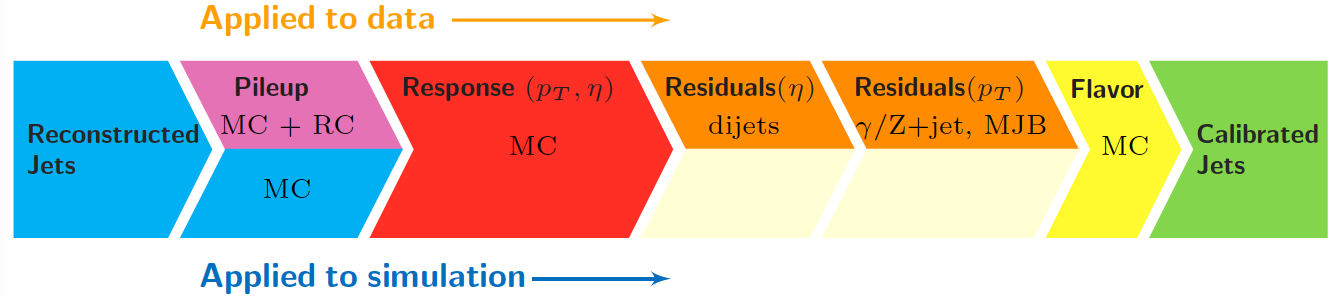
\includegraphics[width=.8\textwidth]{JEC_levels.png}
\caption{Overview of the jet energy calibration procedure followed in data and simulation~\cite{CMS-JME-13-004}.}
\label{fig:JECoverview}
\end{figure}

%% The corrections, parametrized as function of \pt and $\eta$ of the jets, are applied following the standard procedure used by most of the CMS analyses \cite{CMS:JEC_2011, CMS-DP-2016-020, CMS-DP-2021-033}.

\paragraph{Jet energy scale\\}
The JES corrections are calculated in the form of a multiplicative factor on the four-momentum of the measured jet,
in order to match the measured energy of each jet to its true energy at the generator level.
The measured jet transverse momentum response is defined as the ratio of the measured jet \pt at the reconstruction step to the generated jet at particle level.
%% These corrections and the corresponding uncertainties are provided centrally by the CMS JetMet group

\Pileup{} offset corrections account for the measured energy of the jet in excess due to
the presence of in-time (IT) and out-of-time (OOT) \pileup{}
%% They are derived from the simulation of QCD multi-jet events processed with or without \pileup{} overlay
and they are applied to both data and MC samples.

Simulated response corrections compensate for the non-linear response in \pt and pseudorapidity
from the calorimeters and tracker coverage and they are parametrized as a function of these jet kinematic variables.

Residual data to Monte Carlo corrections are applied to improve the agreement as a function of the jet $\eta$ and \pt.
The absolute scale of the measured jet \pt response is corrected in data using multi-jet and Drell-Yan plus jets events,
which benefit from the high precision measurement of the \PZ boson and the photon energy in the ECAL.
The residual $\eta$ correction is derived in di-jet events exploiting the \pt imbalance of the di-jet system.

\paragraph{Jet energy resolution\\}
Jet Energy Resolution (JER) corrections introduce a dose of smearing in the simulated jet \pt spectrum
to compensate for data-to-simulation differences due to detector resolution effects.
They are determined in $\PGg/\PZ$ + jets events by fitting the residual of the \pt distribution to a
double-sided Crystall Ball function.
This accounts for a gaussian core due to statistical fluctuations in the deposited energy,
while the tails account for effects such as inactive areas, neutrino emissions in heavy flavour in-flight decays
or punch-though of hadrons beyond the end of the calorimeter.


\subsubsection{L1 prefiring}
\todo{move to chapter 4}
\label{sec:L1Prefiring}
In 2016 and 2017, the gradual timing shift of ECAL was not properly propagated to \Lone trigger primitives (TP)
resulting in a significant fraction of high eta TP being mistakenly associated to the previous bunch crossing~\cite{CMS-TRG-17-001}.
Since \Lone trigger rules forbid two consecutive bunch crossings to fire,
in addition to missing the trigger primitive in the correct bunch crossing,
events can self veto if a significant amount of ECAL energy is found in the region of $2<|\eta|<3$.
This effect is not described by the simulations.

A similar effect is present in the muon system, where the bunch crossing assignment of the muon candidates can be wrong due to the limited time resolution of the muon detectors.
This effect was most pronounced in 2016, but is non-zero for both 2017 and 2018.
The associated prefiring rate is stable for $\pt > 25 \GeV$ but affects the almost entire eta range.
Its magnitude varies between 0\% and a 3\%.

The probability not to prefire (see Equation~\ref{eq:L1prefiring} is calculated for each event and applied as a weight to simulation for 2016 and 2017 samples,
using a software tool developed by CMS \Lone trigger experts.
\begin{equation}
\label{eq:L1prefiring}
w^{pref} = 1 - \Probability(prefire) = \prod_{i\, \in\, \PGg,\, jets,\, \PGm} (1 - \epsilon_i^{pref}(\eta, \pt))
\end{equation}

The Figure~\ref{fig:L1Prefiring} shows the impact of the L1 pre-firing weights on the signal MC.
The uncertainty of the weights is reflected in a shift
on the normalization of the signal sample of around 0.2\usep\%.

\begin{figure}
\subfigure [L1 pre-firing weights]       {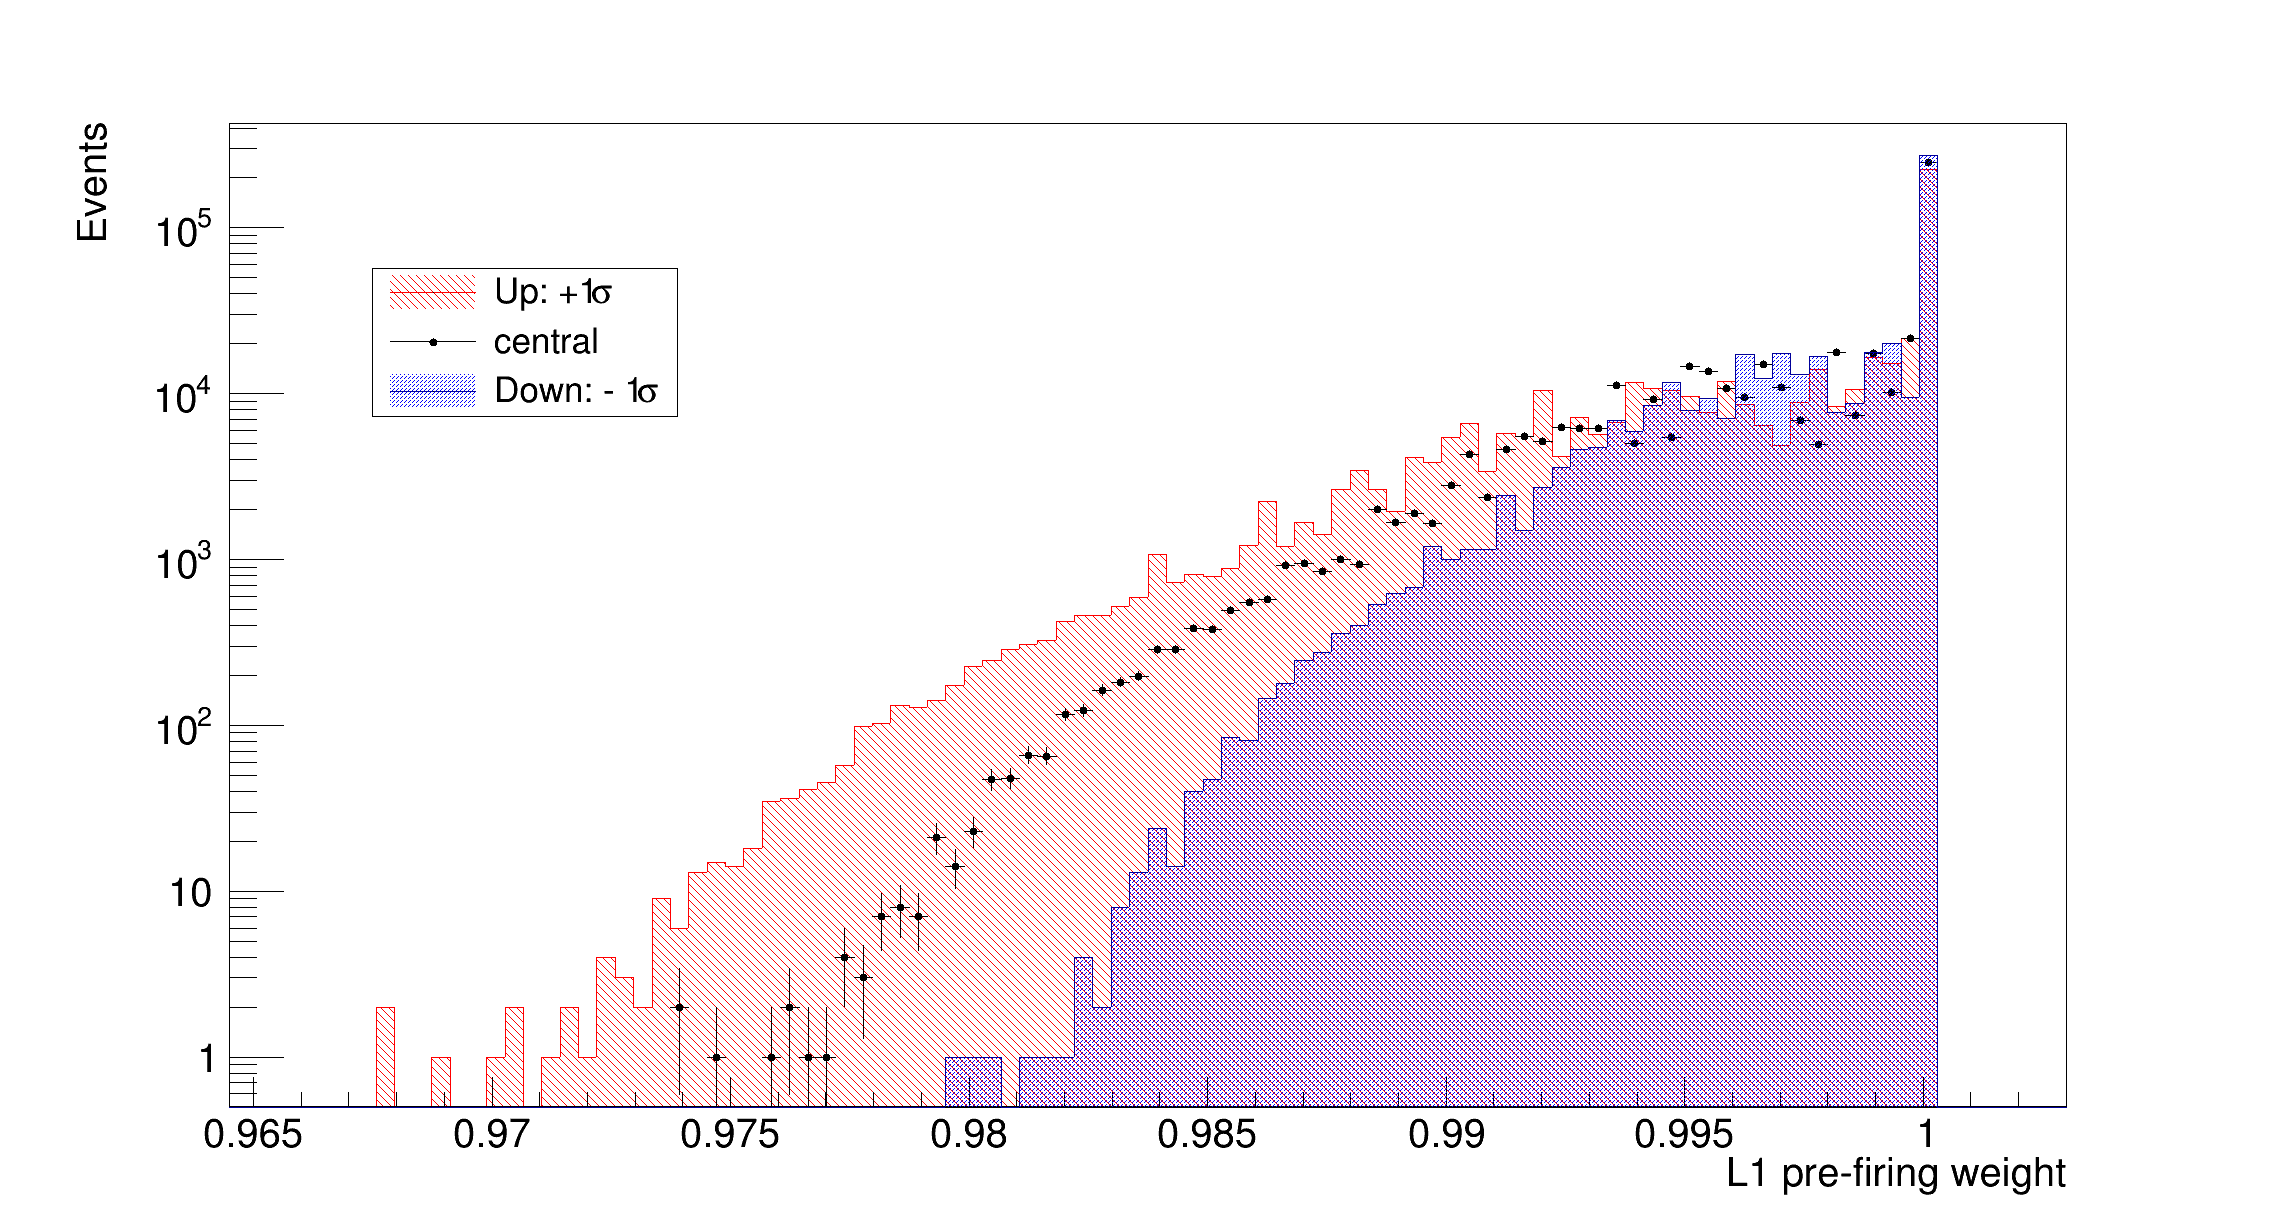
\includegraphics[width=.5\textwidth]{Figures/L1Prefiring_ZZGTo4LG.png}}%
\subfigure [Effect on $m_{4\ell\gamma}$] {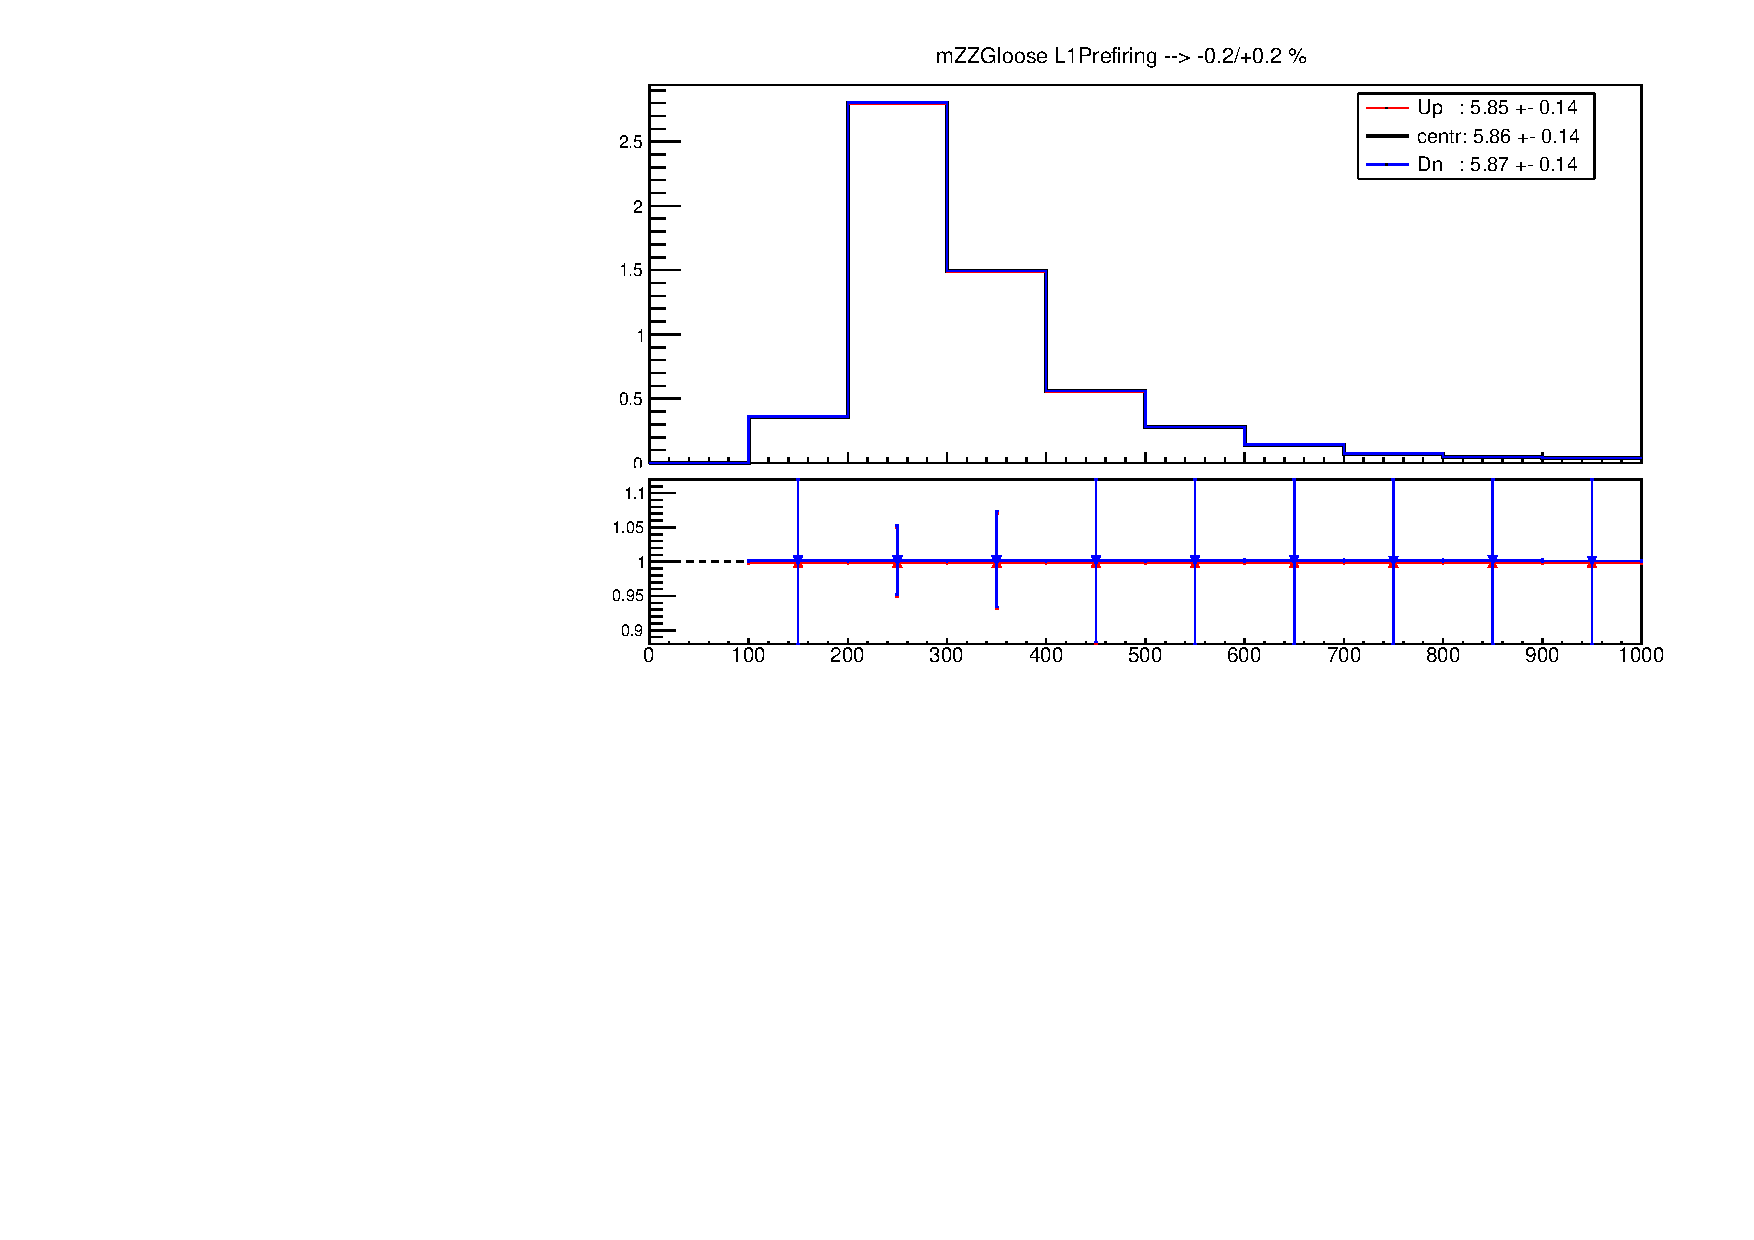
\includegraphics[width=.5\textwidth]{Figures/SYS/SR4P/ZZGTo4LG_mZZGloose_L1Prefiring.pdf}}
\caption{L1 pre-firing weights and their uncertainty on the signal MC in the signal region with four tight leptons and one photon in 2018.
The photon is required to pass the Loose working point of the cut-based ID.}
\label{fig:L1Prefiring}
\end{figure}

